%% LyX 2.0.8.1 created this file.  For more info, see http://www.lyx.org/.
%% Do not edit unless you really know what you are doing.
\documentclass{UNCC-thesis}
\usepackage[T1]{fontenc}
\usepackage[latin9]{inputenc}
\setcounter{secnumdepth}{3}
\usepackage{array}
\usepackage{float}
\usepackage{graphicx}
\usepackage{nomencl}


%===================Package Area========================% 
\usepackage{latexsym} 
\usepackage{amssymb} 
\usepackage{amsmath} 
\usepackage{amsthm} 
\usepackage{graphicx} 
\usepackage{algorithm} 
\usepackage{algorithmic} 
\usepackage{cite} 
\usepackage{fancyhdr} 
\usepackage{lastpage} 
\usepackage{layout} 
\usepackage{subfigure}
%===============End Package Area========================% 
%===============New command Area=========================% 
\newcommand{\DF}[2]{{\displaystyle\frac{#1}{#2}}}% 
\newtheorem{theorem}{Theorem} 
\newtheorem{lemma}[theorem]{Lemma} 
\newtheorem{corollary}{Corollary}
\renewcommand{\algorithmicrequire}{\textbf{Input:}}%Use Input in the format of Algorithm 
\renewcommand{\algorithmicensure}{\textbf{Output:}}%Use Output in the format of Algorithm 
%===============End New command Area=====================% 
%
% the following is useful when we have the old nomencl.sty package
\providecommand{\printnomenclature}{\printglossary}
\providecommand{\makenomenclature}{\makeglossary}
\makenomenclature

\makeatletter

%%%%%%%%%%%%%%%%%%%%%%%%%%%%%% LyX specific LaTeX commands.
%% Because html converters don't know tabularnewline
\providecommand{\tabularnewline}{\\}

\@ifundefined{showcaptionsetup}{}{%
 \PassOptionsToPackage{caption=false}{subfig}}
\usepackage{subfig}
\makeatother

\begin{document}

\pagenumbering{roman}
\fbmatterchapterformat
% Doctype should be either dissertation proposal, dissertation, or thesis.
% If you're getting a master's, specify "thesis" below.  
% If you're getting a PhD, specify "dissertation" below.
\doctype{dissertation}
%%%%%%%%%%%%%%%%     IMPORTANT! IMPORTANT! IMPORTANT! %%%%%%%%%%%%%%%%
% The rules below MUST be followed for the abstract page and chapter titles
% to be correctly formatted.
%
% 1. Only the first letter of the entire title should be capitalized to allow the 
%    title to appear as required by the graduate school on the Abstract page.
% 2. Write chapter titles in ALL CAPS.
%
\title{Efficient Spectrum Management and Rendezvous Schemes for Cognitive Radios}
\author{Ji Li}
\degree{Doctor of Philosophy}
\major{Electrical Engineering}
\publicationyear{2015}

\advisor{Dr. Jiang (Linda) Xie}

% Add the full name and title of all your committee members,
% apart from your advisor, one by one.  The style file expects
% 3 to 5 committee members in addition to your advisor.

\committeeMember{Dr. Yu Wang}
\committeeMember{Dr. Tao Han}
\committeeMember{Dr. Keejae Hong}


% Generate the preliminary title page and copyright page.
\maketitlepage
\makecopyright

\begin{abstract}
You must have an abstract. The content of your abstract goes here. 

The abstract is the briefest possible summary of the work and conclusions
not exceeding one page in length.
\end{abstract}



\chapter{INTRODUCTION}

\section{Cognitive Radio Networks}

\section{Research Motivation}

\section{Overview of Proposed Research}

\section{Proposal Organization}

\chapter{Related Work}
\section{Current Rendevous Schemes}

\chapter{Proposed Research}
\section{Communication Framework for Wide-band Cognitive Radio Networks}

\subsection{System Model}
\label{sec:sys}
We consider that SUs in a CRN can dynamically access a  wide-band spectrum which has a total of $M$ channels indexed from $1$ to $M$, where $M$ is a large number which could be hundreds. There are totally $N$ SUs. Each SU is equipped with only one cognitive radio that cannot perform spectrum sensing and data transmission at the same time. Each SU has a unique ID which can be a  positive integer. Furthermore, we assume that each SU can obtain its available channel set  using a spectrum sensing algorithm \cite{iAkyildiz06NGDSA}. Initially, a SU does not know any information about other SUs, even their unique IDs. A  time-slotted system is adopted in this CRN. In each time slot, a SU either hops onto a channel according to its hopping sequence or stays on its current channel to continue the current communication with another SU. Time slots of different SUs are not necessarily synchronized, which is practical and easy to implement. SUs in the CRN attempt to get  information about other SUs within its transmission range, send packets to other SUs, or receive packets from other SUs. 

In the rest of the paper, we consider the following two scenarios concerning the available channel sets of a SU pair.

\textit{Symmetrical model}: Any SU pair has exactly the same available channel set. According to  \cite{ySong14AQBBP, ySong11AQBPF, ySong15BRACER}, the similarity of the available channel sets between two SUs within one hop is over $85\%$. Thus, this model is reasonable. Moreover, studying this scenario can help us to get solutions for more complicated scenarios.

\textit{Asymmetrical model}: Any SU pair may have different but overlapping available channel sets. This scenario is more practical because of the dynamics caused by PUs' and SUs' traffic and locations.

%Add a new paragraph to define asym/sym model and MTTR ETTR .
\subsection{The Proposed Framework}
\label{sec:framework}
The goal of our proposed framework is to design efficient distributed schemes for each SU to guarantee that it can communicate with other SUs successfully in a wide-band CRN. The framework mainly contains three parts: the initialization process, the process to get control information from neighboring SUs, and the process to send packets to a specific SU. Moreover, the framework does not require a common control channel (CCC) for information exchange. The flow charts of these three parts are shown in Fig. \ref{fig:frame}.
\begin{figure}[hbtp] 
    \begin{center} 
        \includegraphics[width=8cm,height=8cm]{frame.jpg} 
        \caption{The flow charts of our proposed framework.} 
        \label{fig:frame}
    \end{center}  
\end{figure} 

During the initialization process, each SU first divides the whole wide-band spectrum into several virtual spectrum segments (SS). Based on \textbf{Algorithm \ref{al:spl}} (which is explained in Section \ref{sec:split}), each SU can get a unique list containing the number of channels in each SS. We call it the spectrum splitting list (SSL). Using the unique SSL, a SU can obtain the channel index of the start and end channel in each SS (shown in \textbf{Algorithm \ref{al:id}}). Then, each SU  uses its ID (based on \textbf{Algorithm \ref{al:id}}) to determine its home spectrum segment (HS). \textbf{Algorithm \ref{al:id}} is based on mapping all the SUs evenly to the whole spectrum, where we assume that the IDs of SUs are evenly distributed within a certain range. A SU  hops from a channel to another according to the designed channel hopping sequence (based on \textbf{Algorithm \ref{al:generate}} which is explained in Section \ref{sec:seq}) within its HS. Since  SUs are not synchronized, they may be at different positions of the same hopping sequence even they locate in the same HS. This is the initialization process of a SU who just starts in a CRN, as shown in the left of Fig. \ref{fig:frame}.
\begin{algorithm} 
  \caption{The algorithm to determine a SU's home spectrum's index}
  \begin{algorithmic}[1] 
  \label{al:id}
   \REQUIRE ~~\\ 
    The SU's ID $x$.\\
    \ENSURE ~~\\
     The SU's home spectrum's index;
    \STATE Use \textbf{Algorithm \ref{al:spl}} to get the SSL $l$;\\
    \STATE $y = (x-1) \% M+ 1$; //The channel index starts from 1\\
    \STATE $sum=0$;\\
    \FOR{$i=0$ to $l.length-1$}
        \IF{$y > sum\ \mbox{and}\ y \leq sum + l[i]$}
                    \RETURN $i$;\\
                \ENDIF
                \STATE $sum += l[i]$;\\
    \ENDFOR
  \end{algorithmic} 
\end{algorithm}

After the initialization process, a SU  tries to get the control information of all its neighboring SUs which are hopping in the same or different spectrum segments (SSs). We assume that when a SU is not transmitting data packets, it first performs \textbf{Algorithm \ref{al:sym}} or \textbf{Algorithm \ref{al:asym}} (which is explained in Section \ref{sec:seq}) to rendezvous with a SU in its home spectrum segment (HS) and exchange all their known control information about themselves and others. Through this process, each SU can get all the other SUs' information within the same SS and exchange all of their known information. Therefore, after rendezvous and exchange control information with one existing SU in a SS, a  SU can get the control information of all the other SUs in that SS, and all the existing SUs in the SS can also get the information of this SU and all its known information about other SUs. Then, the SU can sequentially hop to each SS, rendezvous with one SU in that SS, and exchange all the  known control information about other SUs by executing \textbf{Algorithm \ref{al:sym}} or \textbf{Algorithm \ref{al:asym}}.  The SU will hop to a next SS only when it has rendezvoused with a SU in the current SS or the time spent in the current SS has already been more than the MTTR of the applied rendezvous scheme (there are no SUs in current SS) . Finally, the  SU will obtain  and update the control information of all other  SUs in the network. A SU can perform the above process periodically to update the control information about other SUs and inform its own change due to the dynamic characteristics of CRNs. The process of getting  the control information of all the neighboring SUs is shown in the middle of Fig. \ref{fig:frame}. 

After the above process of control information exchange, a SU will get some information about other SUs such as their IDs. When a SU wants to send packets to a specific SU, it first uses the receiver's ID  to determine the receiver's home spectrum segment (HS)  (based on \textbf{Algorithm 1}). Then, the SU sender  executes \textbf{Algorithm \ref{al:sym}} or \textbf{Algorithm \ref{al:asym}} to realize rendezvous with the SU receiver in the SU receiver's HS for communications. The flow charts of  communicating with a specific SU is shown in the right of  Fig. \ref{fig:frame}. Because of the spectrum splitting design, the time to obtain control information and to set up communications can be significantly reduced since a SU pair only needs to rendezvous within a specific spectrum segment (SS). In addition, the probability that multiple pairs of SUs rendezvous on the same channel is also reduced since different pairs of SUs may rendezvous in different spectrum segments (SSs). In the following sections, we will give the details of the proposed algorithms in our framework.


\subsection{Proposed Rendezvous Schemes Under the Symmetrical Model}
\label{sec:seq}
A SU sender and receiver have exactly the same available channel set under the symmetrical model. This may not be very practical. However, the algorithms developed under this model are the basis for the asymmetrical  model. 
%\subsubsection{Hopping Sequence Design}

 Under this scenario, each SU has the same available channels in each SS. Each SU hops within its HS according to a channel hopping sequence generated based on its available channel set. Assume that the number of the available channels of both the SU sender and receiver in the SU receiver's HS is $n$. Since a SU sender and receiver have the same available channel set, we use the indexes of all the available channels in a SS, assuming to be from $1$ to $n$, to design the channel hopping sequence. We desire to get a target sequence $s = {s_{1}s_{2}\dots s_{2n}}$ whose length is $2n$ and each channel index from $1$ to $n$  appears exactly twice in $s$. When a SU sender wants to rendezvous with a SU receiver, it first hops to the HS of the SU receiver, generates the same channel hopping sequence as the SU receiver's, and then starts to hop on channel $s_{1}$. Both the SU sender and receiver hop according to the sequence sequentially and circularly, which means that when a SU reaches the end of the hopping sequence, it will continue to hop onto the first channel of the sequence in the next time slot. Assume that the SU receiver is initially on channel $s_{c}, 1\leq c \leq 2n$. We denote $\varepsilon$ as the distance between the SU sender and SU receiver on the channel hopping sequence due to the asynchronization. Therefore, $\varepsilon = c-1$ or $\varepsilon = 2n-(c-1)$ when considering the circulation of the channel hopping sequence. We define the rendezvous sequence (RS) as follows:

\textit{Rendezvous Sequence (RS)}: The sequence $s$ is a RS when no matter what $\varepsilon$ is, within $2n-1$ time slots, the SU sender and receiver will hop on a same channel if both of them hop according to the same hopping sequence sequentially and circularly.

 We use $s$ to represent our desired rendezvous sequence for the rest of the paper.  
We induce  the following lemma to help us design our rendezvous sequence. 
\begin{lemma}
\label{lemma:guar_rend}
Assume that $s_{i} = s_{j} = k, i < j$, $1\leq k\leq n$. If $j - i = k$, $s$ could be a RS.

\end{lemma}
\begin{proof}
We define the \textit{Sequential Distance} of  the element $k$ in the sequence $s$ as $ d_{k} = j-i=k$, and the  \textit{Circular Distance} of  the element $k$ in the sequence $s$ as $ D_{k} = 2n+i-j=2n-k$, which is the number of time slots taken to hop from $s_{j}$ to $s_{i}$ circularly in $s$. We define the distance pair of the channel index $k$ as $p_{k} = (d_{k}, D_{k})$. Since each $d_{k}$ is different and bounded in $[1,n]$ and each $D_{k}=2n-d_{k}$ is different and bounded in $[n,2n-1]$, each $p_{k}$ is different. Assume that initially the SU sender is on channel $s_{1}$ and the SU receiver is on channel $s_{c}$ Therefore, $\varepsilon=c-1$ or $\varepsilon = 2n-(c-1)$, where $0\leq \varepsilon \leq 2n-1$. We ignore the case when $\varepsilon=0$, because under this case, the two SUs are already on the same channel. Thus, we only need to prove our lemma when $1\leq \varepsilon \leq 2n-1$. Since each $p_{i}$ is different, we can definitely find a $p_{t}$ such that $\varepsilon = d_{t}\ \mbox{or}\ D_{t}$. Suppose $s_{i1} = s_{j1} = t, i1 < j1$. Thus, when the SU sender hops on channel $s_{i1}$, it will rendezvous with the SU receiver on channel $s_{j1}$, or when the SU sender hops on channel $s_{j1}$, it will rendezvous with the SU receiver on channel $s_{i1}$. Therefore, sequence $s$ can guarantee a successful rendezvous within $2n-1$ time slots no matter which channel the SU receiver dwells on at the beginning of the rendezvous process.
\end{proof}

In order to efficiently generate $s$, we notice that $s$ has the following properties. 
\begin{lemma}
\label{lemma:no_exist}
When $n = 4t+2$ or $4t+3$, where $t$ is an integer and $t \geq 1$, the rendezvous sequence does not exist.
\end{lemma}
        \begin{proof}
        Designing a rendezvous sequence $s$ as described in \textbf{Lemma \ref{lemma:guar_rend}} is equivalent to dividing  $1,2,\dots, 2n$,  these $2n$ numbers into two lists $l_{l}$ and $l_{r}$, each of which has exactly $n$ different numbers, such that for $k=1,2,\dots,n$, $l_{r}[k] - l_{l}[k] = k$. Then, we have
        \begin{equation}
        \label{eq:sum1}
        \sum^{n}_{k=1}l_{r}[k]-\sum^{n}_{k=1}l_{l}[k]=\sum^{n}_{k=1}k=\DF{n(n+1)}{2},
        \end{equation}
        \begin{equation}
        \label{eq:sum2}
        \sum^{n}_{k=1}l_{r}[k]+\sum^{n}_{k=1}l_{l}[k]=\sum^{2n}_{k=1}k=n(2n+1).
        \end{equation}
        Combining \eqref{eq:sum1} and \eqref{eq:sum2}, we can get 
        \begin{equation}
        \label{eq:sum3}
        \sum^{n}_{k=1}l_{r}[k]=\DF{5n^{2}+3n}{4}.
        \end{equation}
        When $n=4t+2$ or $4t+3$,where $t$ is an integer and $t \geq 1$, the right-hand side of \eqref{eq:sum3} is not an integer which contradicts the fact that it is a sum of $n$ integers.
        \end{proof}
\begin{lemma}
\label{lemma:exist}
When $n=4t$ or $4t+1$, where $t$ is an integer and $t \geq 1$, the rendezvous sequence always exists.
\end{lemma}
        \begin{proof}
        When $n=4$, sequence $"1,1,4,2,3,2,4,3"$ satisfies the requirements of our desired rendezvous sequence.
        When $n=5$, sequence $"1,1,5,2,4,2,3,5,4,3"$ satisfies the requirements of our desired rendezvous sequence.
        When $n > 5$, the proof can be found in the second page of \cite{tSkolem57OCDOI}.
        \end{proof}
Based on the proof of \textbf{ Lemma \ref{lemma:no_exist}} and \textbf{ Lemma \ref{lemma:exist}}, we propose \textbf{Algorithm \ref{al:generate}} to generate our desired rendezvous sequence. Using the channel hopping sequence generated based on \textbf{Algorithm \ref{al:generate}} and \textbf{Lemma \ref{lemma:guar_rend}}, we design the rendezvous algorithm under the symmetrical model as shown in \textbf{Algorithm \ref{al:sym}}.
%\renewcommand\baselinestretch{0.8}\selectfont 
\begin{algorithm} 
  \caption{The algorithm to generate a rendezvous sequence}
  \begin{algorithmic}[1] 
  \label{al:generate}
    \REQUIRE ~~\\
    The number of channels to generate the channel hopping sequence: $n$
    \ENSURE ~~\\
    The desired rendezvous sequence: $s$\\
    \IF{$n<4\ \mbox{or}\ n\%4==2\ \mbox{or}\ n\%4==3$}
                \STATE $s=\phi$;
                \RETURN $s$;
        \ENDIF
    \IF{$n==4$}
                \STATE $s=[1,1,4,2,3,2,4,3]$;
                \RETURN $s$;
        \ENDIF
        \IF{$n==5$}
                \STATE $s=[1,1,5,2,4,2,3,5,4,3]$;
                \RETURN $s$;
        \ENDIF
        \STATE Let $pl=\phi$ be the list of all the position pairs;
        \STATE $m=\lfloor n/4 \rfloor$;
        \IF{$n > 4\ \mbox{and}\ n\%4==0$}
                \STATE Add all pairs $(4m+r, 8m-r)$, for $r=0,1,\dots,2m-1$, to $pl$;
                \STATE Add pairs $(2m+1, 6m)$ and $(2m, 4m-1)$ to $pl$;
                \STATE Add all pairs $(r, 4m-1-r)$, for $r=1,3,\dots,m-1$, to $pl$;
                \STATE Add pair $(m, m+1)$ to $pl$;
                \STATE Add all pairs $(m+2+r, 3m-1-r)$, for $r=0,1,\dots,m-3$, to $pl$;
        \ENDIF
        \IF{$n > 4\ \mbox{and}\ n\%4==1$}
                \STATE Add all pairs $(4m+2+r, 8m+2-r)$, for $r=0,1,\dots,2m-1$, to $pl$;
                \STATE Add pairs $(2m+1 ,6m+2)$ and $(2m+2, 4m+1)$ to $pl$;
                \STATE Add all pairs $(r, 4m+1-r)$, for $r=1,3,\dots,m$, to $pl$;
                \STATE Add pair $(m+1, m+2)$ to $pl$;
                \STATE Add all pairs $(m+2+r, 3m+1-r)$, for $r=1,2,\dots,m-2$, to $pl$;
        \ENDIF
        \FOR{$i=1$ to $n$}
                \STATE $s[pl[i].first] = s[pl[i].second] = pl[i].second - pl[i].first$;
        \ENDFOR
        \RETURN $s$;
  \end{algorithmic} 
\end{algorithm} 
%\renewcommand\baselinestretch{0.8}\selectfont 
\begin{algorithm} 
  \caption{The rendezvous algorithm for a SU sender under the symmetrical model}
  \begin{algorithmic}[1] 
  \label{al:sym}
    \REQUIRE ~~\\ 
    The available channel set $C$ of the SU sender within the SU sender's HS.\\
    \STATE $n$ equals the size of $C$;\\
    \IF{$n\%4==2$ or $n\%4==3$}
                \STATE $m = 4(\lfloor n/4 \rfloor+1)$;\ \ /* To guarantee the existence of the RS */\\
        \ELSE
                \STATE $m = n$;\\
        \ENDIF
    \STATE Generate the channel hopping sequence $s$ based on $m$ and \textbf{Algorithm \ref{al:generate}};\\
    \FOR{$k=1$ to $2m$}
                \IF{$s_{k} > n$}
                        \STATE $s_{k} = s_{k} \% n$;\ \ /* To guarantee $s_{k}$ to be within $n$ */\\
                \ENDIF
        \ENDFOR
    \STATE $i = 1$;\\
    \FOR{$j = 1$ to $2m-1$}
             \IF{The sender receives a CTS packet on channel $C_{s_{i}}$ of the receiver's HS}
             \STATE Perform communications;\\
        \ELSE
              \STATE $i++$;\\
       \ENDIF
    \ENDFOR
  \end{algorithmic} 
\end{algorithm}

We define a round of  channel hopping as  the length of the $2n$ time slots a SU hops sequentially and circularly  according to the channel hopping sequence. An example of rendezvous in one channel hopping round under the symmetrical model is shown in Fig. \ref{fig:sys_ren}. We assume that the number of available channels of a SU pair is $4$. We label each available channel using the index from $1$ to $4$.  Based on \textbf{Algorithm \ref{al:generate}}, their channel hopping sequence is $"1,1,4,2,3,2,4,3"$. Assume that the SU sender starts hopping from the channel  whose index is $s_{1}=1$ and the SU receiver currently stays on the channel whose index is $s_{3}=4$. Then, the SU sender and receiver will rendezvous on the channel whose index is $s_{4}=2$ after $3$ time slots.
\begin{figure}[hbtp] 
    \begin{center} 
        \includegraphics[width=6cm,height=2.3cm]{sys.jpg} 
        \caption{An example of rendezvous under the symmetrical model.} 
        \label{fig:sys_ren} 
    \end{center} 
\end{figure} 

From \textbf{Lemma \ref{lemma:guar_rend}} and \textbf{Algorithm \ref{al:sym}}, we can induce \textbf{Theorem \ref{theo:ettr}}.
\addtocounter{theorem}{-3}
        \begin{theorem}
        \label{theo:ettr}
        Under the symmetrical model, \textbf{Algorithm \ref{al:sym}} can guarantee rendezvous in one round of the channel hopping.  The MTTR of our proposed rendezvous scheme is $2m-1$ and the  ETTR is $m-1$, where n is the number of channels in current SS, $m=n$ if $n\%4 = 0$ or $n\%4=1$, and $m=4(\lfloor n/4\rfloor+1)$ if $n\%4 = 2$ or $n\%4=3$.
        \end{theorem}
        \begin{proof}
        From \textbf{Lemma \ref{lemma:guar_rend}} and \textbf{Algorithm \ref{al:sym}}, the length of our channel hopping sequence is $2m$ and our  rendezvous algorithm can guarantee rendezvous. Thus, according to \textbf{Algorithm \ref{al:sym}}, the \textit{MTTR} is $2m-1$. When the SU sender is on channel $s_{1}$, assume that the SU receiver has equal probability, which is $1/2m$, to be on any channel from $s_{1}$ to $s_{2m}$. According to the proof of \textbf{Lemma \ref{lemma:guar_rend}}, the total number of time slots needed to rendezvous of all possible situations is $\sum_{i=0}^{2m-1}i=m(2m-1)$. Thus, the \textit{ETTR} is $\lfloor  m(2m-1)/2m\rfloor=m-1$.
        \end{proof}
        
\subsection{Under the Asymmetrical Model}
 Under the asymmetrical model, the SU sender and receiver have different available channel sets. The challenge here is that before rendezvous happens, the SU sender does not know the available channel set of the SU receiver. Here, we assume that they have at least one common available channel. Otherwise, they can never achieve a successful rendezvous.\\
 
As a SU pair may have different available channel sets, each SU's channel hopping sequence should  contain all the channels within the SU receiver's HS. We assume that there are totally $n$ channels in the SU receiver's HS which are indexed from $1$ to $n$. The spectrum splitting scheme in Section \ref{sec:split} can guarantee the existence of the channel hopping sequences. We still use  \textbf{Algorithm \ref{al:generate}} to design the basic channel hopping sequence based on these $n$ channels for both the SU sender and receiver. Additionally, we will replace the unavailable channels in the base channel hopping sequence with the ones randomly chosen from the SU sender's or receiver's own available channels to get their own channel hopping sequences. According to \textbf{Lemma \ref{lemma:guar_rend}}, the replacements will not change the property of our channel hopping sequence. Our goal is to design a rendezvous algorithm which can guarantee rendezvous on different channels during several rounds of the channel hopping until rendezvous on the channel which is commonly available for a SU pair. According to the property of the rendezvous sequence, we can simply change the starting position of a SU sender's channel hopping during each channel hopping round. During a new channel hopping round, after changing the  distance between the SU pair's  positions in the channel hopping sequence, the SU sender and receiver can rendezvous on a new channel. The details of the rendezvous algorithm under the asymmetrical model are shown in \textbf{Algorithm \ref{al:asym}}.
%\renewcommand\baselinestretch{0.8}\selectfont 
\begin{algorithm} 
  \caption{The rendezvous algorithm for a SU sender under the asymmetrical model}
  \begin{algorithmic}[1] 
  \label{al:asym}
    \REQUIRE ~~\\ 
    The SU receiver's ID $x$;\\
    The available channel set $C$ of the SU sender in the SU sender's HS.\\
    \STATE Use \textbf{Algorithm \ref{al:spl}} to get the SSL of the whole spectrum band: $l$;
    \STATE Use \textbf{Algorithm \ref{al:id}} to get the index of the HS of the SU receiver: $r$;\\
    \STATE $n=l[r]$;\ \ /* The index starts from $0$ */\\
    \STATE Generate the channel hopping sequence $s$ based on $n$ and \textbf{Algorithm \ref{al:generate}};\\
    \FOR{$i = 1$ to $2n$}
      \STATE $j=i$;\ \ /* The starting hopping position of the current round */\\
             \FOR{$k=0$ to $2n-1$}
             \STATE $\nu = s_{j}$;
             \IF{$\nu \notin C$}
                 \STATE Let $\nu$ be a randomly chosen channel in $C$;
             \ENDIF
             \IF{The rendezvous on $\nu$ succeeds}
                  \STATE Perform communications;\\
             \ELSE
                  \STATE $j++$;\\
                  \IF{$j>2n$}
                        \STATE $j=1$; /* Circularly hopping */\\
                  \ENDIF
             \ENDIF
           \ENDFOR
    \ENDFOR
  \end{algorithmic} 
\end{algorithm}

An example of rendezvous under the asymmetric model is shown in Fig. \ref{fig:asys_ren}. Assume that the available channels of the SU sender are $\{1,2\}$ and the available channels of the SU receiver are $\{1,3\}$. Assume that $n=4$, so the base channel hopping sequence is $"1,1,4,2,3,2,4,3"$. The SU sender starts from channel $s_{1}=1$ and we assume that the SU receiver is on channel $s_{3}=4$. 
During the first round of channel hopping, after the random replacement process, the channel hopping sequences for the SU sender and SU receiver are $"1,1,2,2,1,2,2,2"$ and $"3,3,3,1,3,3,1,1"$, respectively. According to the channel hopping sequences, the SU sender and receiver do not rendezvous on the same channel for the first  round. Then, the SU sender continues the second round of rendezvous by starting from channel $s_{2}=1$ and the base channel hopping sequence will be $"1,4,2,3,2,4,3,1"$. However, the SU receiver will keep using the base rendezvous sequence $"1,1,4,2,3,2,4,3"$ during the second round. Then, during the second round, after the random replacement process, the channel hopping sequences for the SU sender and SU receiver are $"1,1,2,2,2,1,2,1"$ and $"3,3,3,3,1,3,1,1"$, respectively. Finally, the SU sender and receiver rendezvous on channel $1$ which is available for both of them at the end of the second round after $15$ time slots.
\begin{figure}[hbtp] 
    \begin{center} 
        \includegraphics[width=8cm,height=2.1cm]{asys.jpg} 
        \caption{An example of rendezvous under the asymmetrical model.} 
        \label{fig:asys_ren} 
    \end{center}  
\end{figure} 

According to the conclusions under the symmetrical model and \textbf{Algorithm \ref{al:asym}},   we can induce \textbf{Theorem \ref{theo:ettr_asym}}.
%\addtocounter{theorem}{-3}
        \begin{theorem}
        \label{theo:ettr_asym}
        Under the asymmetrical model, \textbf{Algorithm \ref{al:asym}} can guarantee rendezvous.  The \textit{MTTR} of the guaranteed rendezvous is $2n(n-G+1)$, and the upper bound of the \textit{ETTR} is approximately  $(2n-1)/p$, where $n$ is the number of channels in current SS, $G$ is the number of common available channels in current SS, and $p$ is the probability that a channel is available for both the SU sender and receiver.
        \end{theorem}
        \begin{proof}
         The length of the designed sequence $s$ is $2n$. According 
         to \textbf{Algorithm \ref{al:asym}} and the proof of \textbf{Lemma \ref{lemma:guar_rend}}, during each channel hopping round, two SUs can meet  on a different available channel. Since there are total $G$ common available channels in current SS, there are at most $n-G+1$ channel hopping rounds before two SUs hop a common available channel. Therefore, the maximum time slots to a successful rendezvous (\textit{MTTR}) is $2n(n-G+1)$.
          
          Since the probability that a channel is available for both the SU sender and receiver is $p$,  the probability that a successful rendezvous does not happen until the $k$th round is $(1-p)^{k-1}p$. Therefore,  
          \begin{align*}
          ETTR & \leq  \sum_{k=1}^{2n}(1-p)^{k-1}pk(2n-1) \\
                  &  =  \left(\DF{1-(1-p)^{2n}}{p}-2np^{2n}\right)(2n-1)\\
                  &  \approx \DF{2n-1}{p}.
          \end{align*}
        \end{proof}
  Note that the $ETTR$ of our proposed rendezvous algorithms linearly increases with $n$. This is much better than other existing rendezvous algorithms under the asymmetrical model whose $ETTR$ is at least $O(n^{2})$ such as the ones in \cite{zLin11JSBCH,  zLin13EJSRA, rGandhi12FRFMC}.

\subsection{Proposed Spectrum Splitting Scheme}
\label{sec:split}
First, our proposed spectrum splitting algorithm is based on the following mathematical truth.

\addtocounter{theorem}{3}
\begin{lemma}
\label{lemma:spl_1_4t2}
For any integer $a = 4t+2, t > 2$, $a$ can be represented as $a=x+y$, where $x =  4u+1, u \geq 1$ and $y = 4v+1, v \geq 1$, $a,t,u,\mbox{and}\ v$ are integers.
\end{lemma}
\begin{proof}
When $a=4t+2, t>2$, 
if $t = 2q$, $q$ is an integer and $q \geq 1$, then $ a = 8q+2$, thus $a=(4q+1)+(4q+1)$.  
If $t = 2q+1, q \geq 1$, then $a = 8q+6$, thus $a=[4(q+1)+1]+(4q+1)$.
\end{proof}

\begin{lemma}
\label{lemma:spl_2_4t3}
For any integer $a = 4t+3, t > 2$, $a$ can be represented as $a=x+y+z$, where $x =  4u+1, u \geq 1$, $y = 4v+1, v \geq 1$, and $z=4w+1$, $a,t,u,v, \mbox{and}\ w$ are integers.
\end{lemma}
\begin{proof}
When $a=4t+3$, 
if $t = 3q$, $q$ is an integer and $q \geq 1$, then $a = 12q+3$, thus $a=(4q+1)+(4q+1)+(4q+1)$.  If $t = 3q+1, q \geq 1$, then $a = 12q+7$, thus $a=[4(q+1)+1]+(4q+1)+(4q+1)$. If $t = 3q+2, q \geq 1$, then $a = 12q+11$, thus $a=[4(q+1)+1]+[4(q+1)+1]+(4q+1)$.\end{proof}

\begin{lemma}
\label{lemma:spl_3_4t}
For any integer $a = 4t, t >= 2$, $a$ can be represented as $a=x+y$, where $x =  4u, u \geq 1$ and $y = 4v, u \geq 1$, $a,t,u,\mbox{and}\ v$ are integers.
\end{lemma}
\begin{proof}
When $a=4t, t>=2$, 
if $t = 2q$, $q$ is an integer and $q \geq 1$, then $ a = 8q$, thus $a=4q+4q$. If $t = 2q+1, q \geq 1$, then $a = 8q+4$, thus $a=4q+4(q+1)$.
\end{proof}

\begin{lemma}
\label{lemma:spl_4_4t1}
For any integer $a = 4t+1, t >= 2$, $a$ can be represented as $a=x+y$, where $x =  4u, u \geq 1$ and $y = 4v+1, v \geq 1$, $a,t,u,\mbox{and}\ v$ are integers.
\end{lemma}
\begin{proof}
When $a=4t+1, t>=2$, 
if $t = 2q$, $q$ is an integer and $q \geq 1$, then $ a = 8q+1$, thus $a=4q+(4q+1)$.   
If $t = 2q+1, q \geq 1$, then $a = 8q+5$, thus $a=4(q+1)+(4q+1)$.
\end{proof}

Let $\theta$ be the minimum number of channels in a SS. We will discuss how to choose the value of $\theta$ in Section \ref{sec:performance} through simulation results. Given $\theta$, SUs can execute \textbf{Algorithm \ref{al:spl}} to determine the SSL.

\begin{algorithm} 
  \caption{The algorithm to determine the number of channels in each spectrum segment}
  \begin{algorithmic}[1] 
  \label{al:spl}
    \REQUIRE ~~\\ 
    The total number of channels in the whole spectrum band: $M$; the threshold of the minimum number of channels in each spectrum segment: $\theta$
    \ENSURE ~~\\
    The SSL: $l$
    \STATE Initialize $l$ as an empty list;\\
    \STATE Initialize $Q$ as an empty queue;\\
    \STATE $Q.push(M)$;\\
    \WHILE{$Q$ is not empty}
         \STATE Let $\omega$ be the element in $Q$'s head;\\
         \STATE  Pop $\omega$ out of $Q$;\\
         \STATE Use \textbf{Lemma \ref{lemma:spl_1_4t2}} to \textbf{Lemma \ref{lemma:spl_4_4t1}} to represent $\omega$ using a set of numbers so that $\omega$ is the sum of these numbers; Let the set be $A$;\\
         \IF{for each element $\beta \in A$, $\beta \geq \theta$}
             \STATE Push all the elements in $A$ into $Q$;\\
         \ELSE
                \STATE Add $\omega$ to $l$;\\
         \ENDIF
    \ENDWHILE
    \RETURN $l$;
  \end{algorithmic} 
\end{algorithm}

Based on \textbf{Lemma \ref{lemma:spl_1_4t2}} to \textbf{Lemma \ref{lemma:spl_4_4t1}} and \textbf{Algorithm \ref{al:spl}}, each SU can use the same scheme to split the whole spectrum which guarantees the existence of our designed channel hopping sequence in each spectrum segment. An example of our spectrum splitting scheme is that when $M=100$ and $\theta=20$, the SSL is $[28,24,24,24]$ and each element in this SSL can guarantee the existence of our rendezvous sequence according to \textbf{Lemma \ref{lemma:exist}}.

\section{Rendezvous Schemes with Multiple Cognitive Radios}
\subsection{System Model And Problem Description}
\label{sec:pro}
In this paper, we assume that there are totally $N$ SUs and $N_{p}$ PUs coexisting. There are totally $M$ channels that all the SUs and PUs can access.  Each SU is equipped with a GPS  which can get its location coordinates. Furthermore, each SU is equipped with exactly $R$  homogeneous
half-duplex cognitive radios. Therefore, a cognitive radio cannot send and receive signals simultaneously. We assume that for a SU, all its cognitive radios use the same transmission power and have the same interference range.\\

\vspace{-0.4cm}There is no CCC in the network through which all SUs can exchange their control information. Before the initialization process of a CRN, each SU does not know any information about other SUs, which is a very practical assumption. A time-slotted system is deployed among all SUs and they do no need to be strictly synchronized.\\

\vspace{-0.4cm}A channel hopping scheme is adopted for the rendezvous process. During a rendezvous process, each cognitive radio of a SU hops to a  channel chosen from its available channel set, senses the current availability of the channel, and sends an RTS packet or waits for an RTS packet from another SU. Therefore, each time slot includes the sensing phase and the sending or receiving phase during the rendezvous process. According to existing rendezvous schemes, a successful rendezvous occurs when  two SUs hop to a common available channel at the same time slot, but the process of sending an RTS packet and receiving a CTS reply is not considered. In this paper we define this kind of rendezvous as  \textit{channel rendezvous}. This may not be a problem when one SU is always the sender while the other is the receiver, which means that there is an explicit send-or-receive relationship between the two SUs. Under this scenario, after one SU sends an RTS packet,  if the other SU receives the RTS packet and replies a CTS packet, the rendezvous succeeds. \\

\vspace{-0.4cm}However, during the initialization phase of a CRN, each SU may want to rendezvous with other SUs to exchange control information. There is no explicit role for a SU, since it cannot know if other SUs are senders or receivers currently. If two SUs hop to a common available channel and they both have their transceivers on, none of them can receive the RTS packets, which can fail a successful rendezvous. Furthermore, each SU does not know if its target SU is on the current common available channel and is sending or receiving  in the current time slot. Practically, only when the two SUs hop to a common available channel and when one SU is sending  while the other is trying to receive on that channel, a successful rendezvous can finally happen. In this paper, we denote this kind of rendezvous as  \textit{link rendezvous}. Therefore, when a SU is equipped with multiple cognitive radios, during a rendezvous process, the SU should not only consider which available channel each cognitive radio should tune to but also determine that each radio should be in the sending or receiving mode. We call this problem as the \textit{send-or-receive problem} in a rendezvous scheme.\\

\vspace{-0.4cm}For the $i$th SU with $R$ cognitive radios, during time slot $t$ of a rendezvous process, it generates a \textit{task allocation list} $\mathbb{A}^{t}_{i} = {(c^{t}_{i1}, s^{t}_{i1}), (c^{t}_{i2}, s^{t}_{i2}), \dots, (c^{t}_{iR}, s^{t}_{iR})}$, where $1\leq c^{t}_{iu} \leq M$, $s^{t}_{iu} = 1$ (send) or $s^{t}_{iu} = 0$ (receive), and $(c^{t}_{iu}, s^{t}_{iu})$ is called a \textit{task pair} for the $u$th cognitive radio of the $i$th SU during time slot $t$. We also denote $C_{i}^{t}$ as the available channel set of the $i$th SU during  time slot $t$. We define  \textit{link rendezvous} as follows.\\

\vspace{-0.4cm}\textit{Link Rendezvous}: A successful link rendezvous between the $i$th SU and the $j$th SU during time slot $t$ requires that there exists a task pair $(c^{t}_{iu}, s^{t}_{iu})$ for the $u$th cognitive radio of the $i$th SU and a task pair $(c^{t}_{jv}, s^{t}_{jv})$ for the $v$th cognitive radio of the $j$th SU such that $c^{t}_{iu} \in C^{t}_{i}$, $c^{t}_{jv} \in C^{t}_{j}, c^{t}_{iu} = c^{t}_{jv}$, and $s^{t}_{iu}\ \mbox{XOR}\ s^{t}_{jv} = 1$.\\

\vspace{-0.4cm}Moreover,  we can notice that $\mathbb{A}^{t}_{i}$ should satisfy the following constraints:
\begin{enumerate}
\item No two task pairs $(c^{t}_{iu}, s^{t}_{iu})$ and $(c^{t}_{iv}, s^{t}_{iv})$ satisfy that $c^{t}_{iu} = c^{t}_{iv}$ and $s^{t}_{iu} = s^{t}_{iv} = 1$, which means that two cognitive radios of the same SU cannot send RTS packets simultaneously on the same channel.
\item No two task pairs $(c^{t}_{iu}, s^{t}_{iu})$ and $(c^{t}_{iv}, s^{t}_{iv})$ satisfy that $c^{t}_{iu} = c^{t}_{iv}$ and $s^{t}_{iu}\ \mbox{XOR}\ s^{t}_{iv} = 1$, which means that when one cognitive radio of a SU is sending an RTS packet, there should be no  other cognitive radio of the same SU that is trying to receive RTS packets on the same channel.
\end{enumerate}

Therefore, the problem is how to generate a \textit{task allocation list} $\mathbb{A}$ for each SU to realize a fast and guaranteed rendezvous considering the \textit{send-or-receive problem}.

\subsection{Rendezvous Schemes Without Any Information}
\label{sec:rend}
In this section, we discuss the blind rendezvous problem between two SUs when considering multiple cognitive radios and the \textit{send-or-receive problem}. At the beginning of the initialization phase of a CRN, each SU does not know any information about other SUs. Therefore, each SU can only perform a blind rendezvous process based on its local information to set up links with other SUs. However, previous research works only focus on designing the channel-hopping sequence so that the two SUs can hop to a common available channel at the same time, while ignore the \textit{send-or-receive problem}, especially when each SU is equipped with multiple cognitive radios. Our goal is to generate a \textit{task allocation list} for each SU during each time slot based on an existing channel hopping sequence so that two SUs can achieve a successful \textit{link  rendezvous} within bounded time slots.

\subsection{A Basic Solution}
Our proposed basic link rendezvous scheme is to generate a \textit{task allocation list} $\mathbb{A}$ for each SU during each time slot based on an existing channel hopping sequence which can guarantee a successful \textit{channel rendezvous} within bounded time slots. Given a specific channel hopping sequence ( e.g., the jump-stay channel hopping sequence in \cite{zLin11JSBCH}), we denote the channel-hopping sequence for the $j$th radio of the $i$th SU as $\mathbb{S}_{ij}$, and the element in $\mathbb{S}_{ij}$ at time slot $t$ as $\mathbb{S}^{t}_{ij}$. After $\mathbb{S}_{ij}$ is  generated,  for the task allocation list $\mathbb{A}^{t}_{i}$, all the values of $c^{t}_{i1}, c^{t}_{i2}, \dots, c^{t}_{iR}$ are determined as $c^{t}_{i1} = \mathbb{S}^{t}_{i1}, c^{t}_{i2} = \mathbb{S}^{t}_{i2}, \dots, c^{t}_{iR} = \mathbb{S}^{t}_{iR}$. Therefore, the next step is to set the binary values of $0$ or $1$ to $s^{t}_{i1}, s^{t}_{i2}, \dots, s^{t}_{iR}$ to guarantee that $\mathbb{A}^{t}_{i}$ satisfy the constraints explained in Section \ref{sec:pro}.\\

\vspace{-0.4cm} For any $c^{t}_{ij}, 1\leq j \leq R$, if $c^{t}_{ij}$ appears more than once among all the $R$ radios, which means that more than one radio will hop on channel $c^{t}_{ij}$ during time slot $t$, the radios allocated to channel $c^{t}_{ij}$ should wait for RTS packets according to the constraints in Section \ref{sec:pro}   Other radios will randomly choose sending or receiving roles to themselves.\\

\vspace{-0.4cm}Here is an example of the $0-1$ allocation solution. Assume that $R = 5$ and $c^{t}_{i1} = 1, c^{t}_{i2} = 3, c^{t}_{i3} = 3, c^{t}_{i4} = 2, c^{t}_{i5} = 1$. Since channel $3$ appears twice, $s^{t}_{i2} = 0$ and $s^{t}_{i3} = 0$, which means that the second and third radio should wait for RTS packets during the current time slot on channel $3$. Since channel $1$  also appears twice, $s^{t}_{i1} = 0$ and $s^{t}_{i5} = 0$, which means that the first and fifth radio should also wait for RTS packets during the current time slot on channel $1$. For the fourth radio, we can randomly set $s^{t}_{i4} = 1$.  Finally, the generated \textit{task allocation list} for the $i$th SU during time slot $t$ is $\mathbb{A}^{t}_{i} = \{(c^{t}_{i1} = 1, s^{t}_{i1} = 0), (c^{t}_{i2} = 3, s^{t}_{i2} = 0), (c^{t}_{i3} = 3, s^{t}_{i3} = 0), (c^{t}_{i4} = 2, s^{t}_{i4} = 1), (c^{t}_{i5} = 1, s^{t}_{i5} = 0)\}$.\\

\vspace{-0.4cm}The details of our proposed rendezvous scheme for the $i$th SU is shown in \textbf{Algorithm \ref{al:basic}}.\\

\begin{algorithm} 
  \caption{The basic rendezvous algorithm considering the send-or-receive problem}
  \begin{algorithmic}[1] 
  \label{al:basic}
    \REQUIRE ~~\\ 
    The number of cognitive radios: $R$\\
    The current time slot: $t$\\
    A pre-designed channel-hopping sequence $\mathbb{S}$
    \STATE Assume that the $j$th radio starts the channel hopping at time $t_{j}$;
    \FOR{$j = 1$ to $R$}
      \STATE $c^{t}_{ij} = \mathbb{S}_{t+t_{j}}$;
    \ENDFOR
    \FOR{$j = 1$ to $R$}
      \IF{$c^{t}_{ij}$ appears more than once}
        \STATE $s^{t}_{ij} = 0$;
     \ELSE
        \STATE $s^{t}_{ij}$ is randomly set to be either $0$ or $1$;
      \ENDIF
      \STATE Tune the $j$th radio to channel $c^{t}_{ij}$;
      \IF{$c^{t}_{ij} \in C^{t}_{i}$ and $s^{t}_{ij} = 1$}
        \STATE Send an RTS packet on channel $c^{t}_{ij}$;
      \ELSE
        \STATE Wait for an RTS packet on channel $c^{t}_{ij}$;
      \ENDIF
    \ENDFOR
  \end{algorithmic} 
\end{algorithm}

Based on \textbf{Algorithm \ref{al:basic}}, we can get  \textbf{Theorem \ref{the:basic}}.
\begin{theorem}
\label{the:basic}
Algorithm \ref{al:basic} can guarantee a successful \textbf{channel} rendezvous, and the generated \textit{task allocation list} $\mathbb{A}^{t}_{i}$ can satisfy the constraints in Section \ref{sec:pro}
\end{theorem}
\begin{proof}
  Since each cognitive radio of the $i$th SU hops following a pre-defined channel hopping sequence which can guarantee a successful channel rendezvous, our proposed scheme can also guarantee a successful channel rendezvous between two SUs as long as two of their radios achieve a channel rendezvous. Furthermore, according to \textbf{Algorithm \ref{al:basic}}, if multiple radios hop to a same channel,  all of them will wait for RTS packets. Therefore, all the constraints in Section \ref{sec:pro} can be satisfied.
\end{proof}

\subsection{The Enhanced Rendezvous Scheme}
One problem of the basic rendezvous scheme is that multiple radios may all use   one same channel to receive RTS packets, if they all hop to the same channel simultaneously. Therefore, the cognitive radios of a SU are not well utilized. For example, when each SU is equipped with $4$ cognitive radios, if $3$ of them hop to channel $1$ and the last radio hops to channel $2$ at the same time, under the basic scheme it is equivalent to just using two radios during the current time slot. In this section, we propose an enhanced rendezvous scheme, considering multiple cognitive radios and the \textit{send-or-receive problem}, which can well utilize all the radios of a SU during each time slot to achieve a fast \textit{link rendezvous}.\\

\vspace{-0.4cm}The basic idea of our proposed enhanced rendezvous scheme is to split the total $M$ channels into several continuous groups. Each group has exactly $R$ consecutive channels, where $R$ is the number of cognitive radios of a SU. If $M$ mod $R \neq 0$, then sequentially add channel $1$, $2$, \dots, $R-1$ to the last group until the number of channels is $R$. There is an example in Fig. \ref{fig:group} when $M = 10$, $R = 4$, the generated $\lceil\DF{10}{4}\rceil = 3$ channel groups are $\{1,2,3,4\}$, $\{5,6,7,8\}$, and $\{9,10,1,2\}$.\\
\begin{figure}[hbtp] 
    \begin{center} 
      \includegraphics[width=8cm,height=3cm]{group.eps} 
      \caption{An example of generating all channel groups.} 
    \label{fig:group} 
    \end{center}   
\end{figure} 

\vspace{-0.3cm}We denote $M_{s} = \lceil\DF{M}{R}\rceil$ as the total number of channel groups,  $\mathcal{G} = \{G_{1}, G_{2}, \dots, G_{M_{s}}\}$ as the set of all the channel groups, and $G_{i} = \{g_{i1}, g_{i2}, \dots, g_{iR}\}$ as the channels in the $i$th channel group. As all SUs are equipped with exactly $R$ cognitive radios and can access totally $M$ channels, they can generate the same $\mathcal{G}$ independently. For a SU, it applies $M_{s}$ rather than the number of all channels $M$ to generate a hopping sequence, based on an existing channel hopping sequence generating algorithm. We denote this sequence as the \textit{channel-group hopping sequence} (CGHS).\\

\vspace{-0.4cm}Our basic idea is to assign each cognitive radio with a different current available channel during each time slot. During time slot $t$, if the $i$th SU hops to the $j$th channel group, it allocates current available channels  in $G_{j}$ sequentially to its $R$ cognitive radios. If some channels become unavailable during the current slot which makes the total available channels in $G_{j}$ are not enough for all $R$ radios, the SU also allocates the available channels in the next channel groups until each of the $R$ radios is allocated with a different current available channel. If the number of available channels among the total $M$ channels is less than $R$, then allocate each of them to a radio and let the rest radios keep silent during the current time slot. Here is an example when $M = 10$, $R = 3$, and the available channels in each channel group are $\{2,3\}$, $\{5\}$, $\{7,9\}$,  and $\{10,2\}$. Assume that a SU hops to the second channel group during the current time slot according to the CGHS. The $3$ allocated available channels are channel $5$ from the second channel group and channel $7,9$ from the third channel group.\\

\vspace{-0.4cm}The last step is to solve the \textit{send-or-receive problem}. Note that this problem is equivalent to design a binary string of length $R$ containing only  $0$ or $1$. We define such a string of length $R$ as $\beta_{R}$. Therefore, during time slot $t$, solving the \textit{send-or-receive problem} for the $i$th SU is equivalent to designing a binary string $\beta^{t}_{iR}$. We derive the following lemmas regarding a successful \textit{link rendezvous} between the $i$th and $j$th SU based on $\beta^{t}_{iR}$ and $\beta^{t}_{jR}$.\\

\addtocounter{theorem}{-1}
\begin{lemma}
\label{le:guarantee}
A necessary condition of a successful \textbf{link} rendezvous between the $i$th and $j$th SU during time slot $t$ is that $\beta^{t}_{iR}\ \mbox{XOR}\ \beta^{t}_{jR} > 0$, if we regard $\beta^{t}_{iR}$ and $\beta^{t}_{iR}$ as the binary representations of two integers.
\end{lemma}
\begin{proof}
If $\beta^{t}_{iR}\ \mbox{XOR}\ \beta^{t}_{jR} = 0$, i.e., every bit of the two binary strings is the same, there does not exist a send-and-receive pair between the two SUs which can  guarantee successfully sending and receiving RTS packets. However, if $\beta^{t}_{iR}\ \mbox{XOR}\ \beta^{t}_{jR} > 0$, there are at least two corresponding bits that are different and they can make one radio of a SU send and one radio of the other SU  receive.\end{proof}

The challenge of designing $\beta^{t}_{iR}$ is that the two SUs do not know any information about each other before a successful rendezvous. Our goal is to find a good distributed scheme to generate $\beta$ so that $\beta^{t}_{iR}\ \mbox{XOR}\ \beta^{t}_{jR} = 0$ happens as less as possible. The following lemma can help us design a well performed $\beta_{R}$.\\
\begin{lemma}
\label{le:equal1}
Two different binary strings $\beta_{iR}$ and $\beta_{jR}$, always satisfy $\beta_{iR}\ \mbox{XOR}\ \beta_{jR} > 0$, as long as they are the binary representations of two different integers from the range $[0, 2^{R}-1]$.
\end{lemma}
\begin{proof}
If $\beta_{iR}\ \mbox{XOR}\ \beta_{jR} = 0$, the decimal representations of the two binary strings should be the same, as each bit of the two strings is the same, which contradicts the fact that they represent two different numbers.
\end{proof}

The details of our proposed enhanced rendezvous scheme for the $i$th SU is shown in \textbf{Algorithm  \ref{al:enhanced}}.\\

\begin{algorithm} 
  \caption{The enhanced blind rendezvous algorithm considering the send-or-receive problem}
  \begin{algorithmic}[1] 
  \label{al:enhanced}
    \REQUIRE ~~\\
    SU's unique ID $i$\\
    The number of cognitive radios $R$\\
    The current time slot $t$\\
    An existing channel hopping sequence generating algorithm\\
    \STATE Get the list of channel groups $\mathcal{G}$;
    \STATE Based on $M_{s} = \lceil\DF{M}{R}\rceil$, generate a group hopping sequence $\mathbb{S}_i$;
    \STATE Current channel group id $k$ = $\mathbb{S}_i^{t}$;
    \FOR{$j = 1$ to $R$}
        \STATE $c^{t}_{ij} = $ an available channel in $G_{k}, G_{k+1}, \dots$;
    \ENDFOR
    \STATE Randomly choose an integer from the range $[0, 2^{R}-1]$;
    \STATE Get the binary representation $\beta_{R}$ of length $R$ of the chosen number;
    \FOR{$j = 1$ to $R$}
      \IF{$\beta_{R}[j] = 1$}
      \STATE $s^{t}_{ij} = 1$;
      \ELSE
      \STATE $s^{t}_{ij} = 0$;
      \ENDIF
    \ENDFOR
    \FOR{$j = 1$ to $R$}
      \IF{$s^{t}_{ij} = 1$}
        \STATE Turn on the transceiver of the $j$th radio and send an RTS packet on channel $c^{t}_{ij}$;
      \ELSE
        \STATE Turn on the receiver of the $j$th radio and stay on channel $c^{t}_{ij}$ waiting for RTS packets;
      \ENDIF
    \ENDFOR
  \end{algorithmic} 
\end{algorithm}

Based on \textbf{Lemma \ref{le:equal1}} and \textbf{Algorithm \ref{al:enhanced}}, we can get \textbf{Theorem \ref{th:enhanced}}.\\

\addtocounter{theorem}{-1}
\begin{theorem}
\label{th:enhanced}
The enhanced rendezvous scheme in Algorithm \ref{al:enhanced} can guarantee a successful \textit{\textbf{channel} rendezvous}. The probability that two SUs independently choose the same binary string for the send-or-receive problem, which may fail a \textit{link rendezvous}, is  $\DF{1}{2^{R\eta}}$, where $R$ is the number of cognitive radios each SU is equipped with and $\eta$ is the number of times that two radios of the two SUs hop to a common available channel during a blind rendezvous process.\end{theorem}
\begin{proof}
  We define a channel group between two SUs as a valid group if there is a common available channel in it. As long as two SUs have at least one common available channel, there is a valid group between them as they split all the channels into the sam channel groups. Therefore, the two SUs will hop to a valid group as long as they follow the hopping sequence which can guarantee a successful \textit{channel rendezvous} on a common available channel. According to \textbf{Algorithm \ref{al:enhanced}}, two SUs have the same send-or-receive allocations only when they choose the same random integer from the range $[0, 2^{R}-1]$. The probability that two SUs independently choose the same integer from  $[0, 2^{R}-1]$ is $\DF{1}{2^{R}}\times\DF{1}{2^{R}} = \DF{1}{2^{2R}}$. There are totally $2^{R}$ different integers from $[0, 2^{R}-1]$. Therefore, the final probability of a link rendezvous failure is $(\DF{1}{2^{2R}}\times 2^{R})^{\eta} = \DF{1}{2^{R\eta}}$.
\end{proof}

\subsection{Rendezvous Scheme with Some Information}
\label{sec:renWithInfo}
In the last two proposed rendezvous schemes, we consider the scenario that a SU does not know any information about other SUs. However, if a SU has known the control information about some other SUs such as their locations and current available channels, the situation will be different when the SU generates the \textit{task allocation list}. We assume that when two SUs rendezvous successfully, they  exchange all of their known control information about other SUs and themselves. When considering multiple cognitive radios, several SUs may be connected  together through some radios and form a connective graph (for each two SUs, there is a path for any one of them to reach the other one). After information exchange,  how to optimally allocate the rest available channels to current free radios based on the obtained information about the already connected SUs to perform rendezvous with other non-connected SUs is a problem. Especially, if two SUs are located within the interference range of each other, when they allocate the same channel to their free radios, the allocation is invalid due to the interference. Therefore, when  SUs are allocating channels to their free radios, they should attempt to reduce invalid channel allocations. We call this as the \textit{channel allocation problem} during a rendezvous process when considering multiple cognitive radios.\\

\vspace{-0.4cm}An example is shown in Fig. \ref{fig:exampleAlloc}.  During the current time slot, SU \textit{A} has rendezvoused with SU \textit{B} on their commonly available channel $1$ and SU \textit{C} has rendezvoused with SU \textit{B} on their commonly available channel $2$. We assume that each SU is equipped with $3$ cognitive radios, and during the current time slot, their available channel sets are $\{1,3,4\}$, $\{1,2,4\}$, and $ \{1,2,3\}$. After information exchange, all the $3$ SUs know the location and current available channel set of each other. For SU \textit{A} and \textit{C}, there are two remaining free cognitive radios, but SU \textit{B} only has one more free radio to utilize. We assume that they are all located within the interference range of each other, which means that any two of them cannot use the same channel in order to avoid interference. Therefore, how to allocate the remaining free available channels to the remaining free cognitive radios is a problem, for instance, SU \textit{A} and \textit{C} cannot use channel $3$ simultaneously.\\
\begin{figure}[hbtp] 
    \begin{center} 
      \includegraphics[width=4cm,height=3cm]{fig1.jpg} 
      \caption{An example of the channel allocation problem.} 
    \label{fig:exampleAlloc} 
    \end{center}   
\end{figure} 

\vspace{-0.4cm}
During a time slot, we assume that there are totally $N_{c}$ SUs who can get the information of each other through existing rendezvouses, and each SU is equipped with $R$ cognitive radios. The $i$th SU's remaining available channel set is $C^{'}_{i}$ (some available channels have been used in establishing links such as channel $1$ in the example), its location is represented as a vector $L_{i}$, and the number of remaining radios is $\delta_{i}$.  If a radio of a SU is allocated with an available channel and there is no  other SU within its interference range using the same channel, we denote this kind of radio as a \textit{valid allocated radio}. Our goal is to maximize the total number of \textit{valid allocated radios} among all the $N_{c}$ SUs.\\

\vspace{-0.4cm}
We define the maximum number of SUs that can use channel $i$ simultaneously as the \textit{maximum utilization number} of channel $i$ which is denoted as $\mu_{i}$ and the corresponding set of SUs that can use channel $i$ simultaneously without causing any interference to each other as $\mathbb{B}_{i} = \{\theta_{1}, \theta_{2}, \dots, \theta_{\mu_{i}}\}$, where $\theta_{j}$ is the ID of a SU that can use channel $i$. The first step is to get $\mu_{i}$ and $\mathbb{B}_{i}$ for channel $i$. We will solve this problem based on the following lemma.\\

\begin{lemma}
\label{le:clique}
To get $\mu_{i}$ and $\mathbb{B}_{i}$  is equivalent to solving the maximum clique problem of a corresponding undirected graph $G = \{V, E\}$. 
\end{lemma}

\begin{proof}
The maximum clique problem of an undirected graph $G = \{V, E\}$ is defined as finding a subgraph $G_{m} = \{V_{m}, E_{m}\}\in G$ which has the maximum number of nodes, $V_{m} \in V$, $E_{m} \in E$, and for any two different nodes $u, v\in V_{m}$, there is an edge $(u,v)\in E_{m}$ \cite{iBomze99TMCP}. For channel $i$, we build graph $G = \{V, E\}$ in the following way, $V = \{1,2,\dots,N_{c}\}$, where $N_{c}$ is the number of SUs who know the information of each other; an undirected edge $(u, v) \in E$ exists if SU $u$ and SU $v$ are not located in the interference range of each other; and $i\in C^{'}_{u}$, $i\in C^{'}_{v}$. After establishing $G$, the problem is equivalent to finding a subgraph $G^{'} = \{V^{'},E^{'}\} $ of $G$ with the maximum number of nodes and $\forall u,v\in V^{'}$, $u \neq v$, the edge $(u,v)\in E^{'}$. This is the maximum clique problem of graph $G$.\\
\end{proof}

The maximum clique problem is an NP problem and there are a lot of existing algorithms to solve it \cite{Carraghan90AEAFT, iBomze99TMCP}. Here is an example of getting $\mu_{i}$ and $\mathbb{B}_{i}$ for channel $i$ through solving the maximum clique problem. Assume that channel $i$ is available for SU \textit{A}, \textit{B}, \textit{C}, and \textit{D} simultaneously. SU \textit{A} and SU \textit{D} are located within the interference range of each other. SU \textit{B} and SU \textit{C} are located within the interference range of each other. Therefore, according to the proof of \textbf{Lemma \ref{le:clique}}, the established graph for this example is shown in Fig. \ref{fig:exampleClique}. An edge between two SUs means that they can use channel $i$ simultaneously since they are out of the interference range of each other. The maximum clique of this  graph is very straightforward that $\mu_{i} = 2$ and $\mathbb{B}_{i}$ can be $\{A, B\}$.\\
\begin{figure}[hbtp] 
    \begin{center} 
      \includegraphics[width=3cm,height=3cm]{clique.jpg} 
      \caption{An example of the maximum clique problem.} 
    \label{fig:exampleClique} 
    \end{center}   
\end{figure} 

\vspace{-0.4cm}
Based on \textbf{Lemma \ref{le:clique}}, we give the details of how to get $\mathbb{B}_{i}$ for channel $i$ in \textbf{Algorithm \ref{al:getMaxNum}}.\\

\begin{algorithm} 
  \caption{The algorithm to get $\mathbb{B}_{i}$ for the $i$th channel}
  \begin{algorithmic}[1] 
  \label{al:getMaxNum}
    \REQUIRE ~~\\
    Channel id: $i$\\
    The number of SUs who know the information of each other: $N_{c}$\\
    The set of all the $N_{c}$ SUs' location: $\mathcal{L}=\{L_{1},L_{2},\dots,L_{N_{c}}\}$\\
    The radius of the interference range of all SUs: $I_{r}$\\
    The remaining available channel sets of all $N_{c}$ SUs: $C^{'}_{1}, C^{'}_{2}, \dots, C^{'}_{N_{c}}$\\
    \ENSURE ~~\\
    Channel allocation set for channel $i$: $\mathbb{B}_{i}$\\
    \STATE Initialize a graph $G = (V, E)$ that $V = E = \phi$;
    \STATE $V = \{1, 2, \dots, N_{c}\}$;
    \FOR{$u = 1$ to $N_{c}$}
      \FOR{$v = 1$ to $N_{c}$}
        \IF{$u \neq v$, $i\in C^{'}_{u}$, $i\in C^{'}_{v}$, and $\parallel L_{u}-L_{v}\parallel_{2} \geq I_{r}$}
          \STATE Add an undirected edge $(u, v)$ to $E$;
        \ENDIF
      \ENDFOR
    \ENDFOR
    \STATE Solve the maximum-clique problem of $G$;
    \STATE $\mathbb{B}_{i} = $ the set of nodes which forms the maximum clique of $G$;
    \RETURN{$\mathbb{B}_{i}$}
  \end{algorithmic} 
\end{algorithm}

\vspace{-0.4cm}
Based on \textbf{Algorithm \ref{al:getMaxNum}}, we design a distributed algorithm for each SU in \textbf{Algorithm \ref{al:getChannelSet}} which can allocate available channels to the SU's current free radios to maximize the total number of \textit{valid allocated radios} among all $N_{c}$ SUs.\\

\begin{algorithm} 
  \caption{The distributed algorithm to optimally allocate available channels for the $i$th SU}
  \begin{algorithmic}[1] 
  \label{al:getChannelSet}
    \REQUIRE ~~\\
    The SU's ID: $i$\\
    Current available channel set: $C_{i}$\\
    Other connected SUs' locations and available channel sets\\
    The radius of the interference range of all SUs: $I_{r}$\\
    The number of cognitive radios that have not been allocated with channels: $\delta_{i}$
    \ENSURE ~~\\
    Channel allocation set: $\mathcal{C}^{'}_{i}$\\
    \STATE $l = \phi$;
    \FOR{$j = 1$ to $M$}
      \IF{$j\in C_{i}$}
        \STATE Get $\mathbb{B}_{j}$ through Algorithm \ref{al:getMaxNum};        \STATE $l.append(\mathbb{B}_{j})$;
      \ENDIF
    \ENDFOR
    \STATE Reversely sort $l$ according to $|l[i]|$, where $|.|$ is the size of a set.
    \STATE $\mathcal{C}^{'}_{i} = \phi$;
    \FOR{$j = 0$ to $l.length-1$}
      \IF{$i \in l[j]$ and $\delta_{i} > 0$}
        \STATE Add the corresponding channel ID of $l[j]$ to $\mathcal{C}^{'}_{i}$;
        \STATE $\delta_{i} = \delta_{i} - 1$;
      \ENDIF
      \IF{$\delta_{i} == 0$}
        \STATE break;
      \ENDIF
    \ENDFOR
    \RETURN{$\mathcal{C}^{'}_{i}$}
  \end{algorithmic} 
\end{algorithm}

\vspace{-0.4cm}
Based on \textbf{Algorithm \ref{al:getMaxNum}} and \textbf{Algorithm \ref{al:getChannelSet}}, we can get the following theorem.\\

\addtocounter{theorem}{-1}
\begin{theorem}
\label{th:maxNum}
If there are $N_{c}$ SUs who know the information of each other, after all the SUs execute \textbf{Algorithm \ref{al:getChannelSet}}, the total number of \textit{valid allocated radios} among all SUs  will reach its maximum, and no two SUs who are located within each other's interference range use the same available channel.
\end{theorem}
\begin{proof}
 If the result is not the maximum, there must be a free radio that still can be allocated with a channel without causing interference to other SUs. We assume that the $j$th radio of the $i$th SU can be allocated with channel $k$. We can get $\mathbb{B}_{k}$ from \textbf{Algorithm \ref{al:getMaxNum}} and $\mathbb{B}_{k}$ is not empty. If $i\in \mathbb{B}_{k}$, this contradicts the fact that the $j$th radio of the $i$th SU is still free, because otherwise it should have been allocated with channel $k$ according to \textbf{Algorithm \ref{al:getChannelSet}}. If $i\not\in\mathbb{B}_{k}$, there must be a radio of another SU who has been allocated with channel $k$. If the $j$th radio of the $i$th SU is allocated with channel $k$, there must be interference between the $i$th SU and the one already allocated with channel $k$. Therefore, we cannot allocate any channel to one more free radio after executing \textbf{Algorithm \ref{al:getChannelSet}}.
\end{proof}

Based on \textbf{Algorithm \ref{al:getChannelSet}}, we propose a new rendezvous scheme if each SU knows the control information of each other among all $N_{c}$ SUs. The details are shown in \textbf{Algorithm \ref{al:notBlind}}.\\

\begin{algorithm} 
  \caption{The rendezvous algorithm with some known information}
  \begin{algorithmic}[1] 
  \label{al:notBlind}
    \REQUIRE ~~\\
    Current available channel set: $C$;
    \IF{a SU can get the information from other SUs}
      \STATE Get $\mathcal{C}^{'}$ from \textbf{Algorithm \ref{al:getChannelSet}};
      \STATE Use $\mathcal{C}^{'}$ and \textbf{Algorithm \ref{al:enhanced}} or \textbf{Algorithm \ref{al:basic}} to perform a rendezvous process;
    \ELSE
      \STATE Use $C$ and \textbf{Algorithm \ref{al:enhanced}} or \textbf{Algorithm \ref{al:basic}} to perform a rendezvous process;
    \ENDIF
  \end{algorithmic} 
\end{algorithm}


\section{Rendezvous Scheme Without Predetermined Send or Receiver}
\subsection{System Model And Problem Description}
\label{sec:pro}
In this paper, we assume that there are totally $N$ SUs and $N_{p}$ PUs coexisting. There are totally $M$ channels that all the SUs and PUs can access. Furthermore, each SU is equipped with a
half-duplex cognitive radio. Therefore, a cognitive radio cannot send and receive signals simultaneously. There is no CCC in the network through which all SUs can exchange their control information. Before the initialization process of a CRN, each SU does not know any control information about other SUs, which is a very practical assumption. A time-slotted system is deployed among all SUs and PUs  and they do no need to be strictly synchronized.\\

\vspace{-0.4cm}
A channel hopping scheme is adopted for the  rendezvous process between two SUs. During a rendezvous process, each SU hops to the current  channel based on a channel hopping sequence, senses the current availability of the channel, and sends an RTS packet or waits for an RTS packet from another SU. Therefore, each time slot includes the sensing phase and the sending or receiving phase during the rendezvous process. According to existing rendezvous schemes, a successful  rendezvous occurs when  two SUs hop to a common available channel at the same time slot, but the process of sending an RTS packet and receiving a CTS reply is not considered. In this paper we define this kind of rendezvous as  \textit{channel rendezvous}. This may not be a problem when one SU is always the sender while the other is the receiver, which means that there is an explicit send-or-receive relationship between the two SUs. Under this scenario, after one SU sends an RTS packet,  if the other SU receives the RTS packet and replies a CTS packet, the rendezvous succeeds. \\

\vspace{-0.4cm}
However, during the initialization phase of a CRN, each SU may try to rendezvous with other SUs to exchange control information. There is no explicit role for a SU, since it cannot know if other SUs are senders or receivers currently. If two SUs hop to a common available channel and their transceivers are both tuning to the sending mode , none of them can receive the RTS packets, which can fail a successful rendezvous. Furthermore, each SU does not know if its target SU is on the current common available channel and is  in the sending or receiving mode  during the current time slot. Practically, only when the two SUs hop to a common available channel and when one SU is sending  while the other is trying to receive on that channel, a successful rendezvous can finally happen. In this paper, we denote this kind of rendezvous as  \textit{link rendezvous}. Therefore, in a \textit{link rendezvous} process without the explicit sender or receiver , a SU  should not only determine the channel it should hop to but also whether tuning its half-duplex radio to the sending or receiving mode during a time slot. We call this problem as the \textit{send-or-receive problem} in a \textit{link rendezvous} scheme. \\

\vspace{-0.4cm}
For the $i$th SU, during time slot $t$ of a link rendezvous process, it generates a \textit{task allocation} $\mathbb{A}^{t}_{i} = (c^{t}_{i}, s^{t}_{i})$, where $1\leq c^{t}_{i} \leq M$, $s^{t}_{i} = 1$ (send) or $s^{t}_{i} = 0$ (receive).  We also denote $C_{i}^{t}$ as the available channel set of the $i$th SU during  time slot $t$. We define  \textit{link rendezvous} as follows.\\

\vspace{-0.4cm}
\textit{Link Rendezvous}: A successful link rendezvous between the $i$th SU and the $j$th SU during time slot $t$ requires that $(c^{t}_{i}, s^{t}_{i})$ and $(c^{t}_{j}, s^{t}_{j})$ satisfy $c^{t}_{i} \in C^{t}_{i}$, $c^{t}_{j} \in C^{t}_{j}, c^{t}_{i} = c^{t}_{j}$, and $s^{t}_{i}\ \mbox{XOR}\ s^{t}_{j} = 1$.\\

\vspace{-0.4cm}
In the following two sections, we propose two different distributed link rendezvous schemes based on two different basic ideas.
\subsection{Basic Link Rendezvous Scheme}
\label{sec:ba_rend}
Our basic idea is that besides the channel hopping sequence, considering the send-or-receive problem,  there is a  \textit{transmission sequence}
$S_i$ for the $i$th SU. $S_i$ only contains $0$ or $1$ values which represent
the sending mode or receiving mode, respectively,  for each SU during each time slot, i.e, If $S_i[t] = 1$,
during the current time slot, the SU should tune its transceiver to the
sending mode, and If $S_i[t] = 0$, during the current time slot, the SU should tune its transceiver to the receiving mode. When tuning to the sending
mode during a time slot, a SU can first send an RTS packet on the current channel and
then tune to the receiving mode waiting for a replied CTS packet. When tuning to the receiving mode, a SU should tune the transceiver to the receiving mode, wait for RTS packets from  other SUs on the current channel, and tune to the sending to reply a CTS packet if it received an RTS packet.\\

\vspace{-0.5cm}
Since we try to design a distributed scheme for each SU, our idea for the basic link rendezvous scheme is to make each SU apply the same  basic transmission sequence $S_b$.
We assume that the length of the  basic transmission sequence $S_b$ is $L$ and each SU circularly hops according to $S_b$, i,e, if the SU hops to the end of $S_b$, it should hop to the first element of $S_b$ during the next time slot.  For example, if the  transmission sequence is $\{1,0,0,1\}$,
the real transmission sequence should be $\{1,0,0,1,1,0,0,1,1,0,0,1\dots\}$. However, since
two SUs are not synchronized and do not know any control information about each other
before a successful link rendezvous, two SUs may follow different  real transmission
sequences even though they all follow the same basic transmission sequence $S_b$. Therefore, for the $i$th SU and $j$th SU, the real transmission
sequence of the $j$th SU $S_j$ should be a circular shift from the $i$th
SU's real transmission sequence $S_{i}$. For example, if the basic transmission sequence $S_b$
is $\{1,0,0,1\}$, $S_{i}$ is $\{1,0,0,1,1,0,0,1,\dots\}$, and $S_{j}$ is $\{1,1,0,0,1,1,0,0,\dots\}$.\\

\vspace{-0.4cm}
We define the element pair $(S^{t}_i, S^{t}_j)$ as the \textit{transmission pair}
of the $i$th and $j$th SU. According to the previous analysis, only when one SU is on sending mode while the
other is on receiving mode, two SUs can successfully finish a RTS and CTS
exchange. Therefore, only the transmission pair $(0,1)$ or $(1,0)$ can result
in a successful link rendezvous. We define $(0,1)$ or $(1,0)$ as the \textit{valid transmission
pair}.  We define the \textit{valid number} $N_v = \mathcal{V}(S_{i},
S_{j})$ as the number  of valid transmission pairs two real transmission
sequences could get within the period $L$, where
\begin{equation}
 \mathcal{V}(S_{i}, S_{j}) = \sum_{k=0}^{L-1}[(S_{i}[k]\ XOR\ S_{j}[k])
== 1].
\end{equation}
Furthermore, the average valid number $\overline{N_v}$ of a basic transmission
sequence $S_b$  is defined as
\begin{equation}
\overline{N_v} = \mathcal{B}(S_b)=\DF{1}{L}\sum_{k=0}^{L-1}\mathcal{V}(S_{i},
\mathcal{H}(S_j, k)),
\end{equation}
where $\mathcal{H}(S_j, k)$ is defined as the function to make $S_j$ perform
$k$ times circularly left shifts. A larger $\overline{N_v}$ means that there are more valid transmission pairs within a period which can make a successful link rendezvous happen with a higher probability. Therefore, our goal is to find the optimal
basic transmission sequence $S_b$ for a given length $L$, which can finally result in 
the largest average valid number $\overline{N_v}$.\\

\vspace{-0.4cm}
To get the optimal basic transmission sequence $S_b$ with length $L$, we first
derive the following lemma:
\begin{lemma}
\label{le:valid1}
For a basic transmission sequence with length $L$, if there are $n$ $1$ elements
in it. The average valid number $\overline{N_v}$ is $2(nL-n^2)/L.$
\end{lemma}
\begin{proof}
Considering all the $L$  scenarios regarding different circular shifts regarding a basic transmission sequence, each $1$ element can generate total
$L-n$ such $(1,0)$ pairs which are valid transmission pairs. Therefore there are total $2n(L-n)$ $(1,0)$ pairs two basic transmission sequences can get. Finally,
the average valid number considering all $L$ different circular shifts 
is    
$2(nL-n^2)/L$.
\end{proof}

\begin{lemma}
\label{le:optimal1}
When the number of $1$  elements in $S_b$ is $\DF{L}{2}$, The average valid number
$\overline{N_v}$ reaches its maximum value $L/2$.
\end{lemma}
\begin{proof}
For a given $L$, $\overline{N_v} = \DF{2}{L}(n_rL-n_r^{2}) = \DF{2}{L}(-(n_r-\DF{L}{2})^{2}+\DF{L^{2}}{4})$.
Therefore, when $n=\DF{2}{L}$, $\overline{N_v}$ reaches the maximum value
$\DF{2}{L}\times \DF{L^2}{4} = \DF{L}{2}$.
\end{proof}

\textbf{Lemma \ref{le:valid1}} indicates that $\overline{N_v}$ is only related
to the number of $1$ elements in $S_b$ regardless of their positions, for a given
$L$. Therefore,  each SU can just generate its own basic transmission sequence of length $L$ which also should contains $\DF{L}{2}$ $1$ elements. We propose a distributed  algorithm for each SU to achieve a successful link rendezvous in \textbf{Algorithm \ref{al:rend1}} in which we let $L$ equal to the number of total channels.
\begin{algorithm} 
  \caption{The basic distribute rendezvous algorithm for each SU}
  \begin{algorithmic}[1] 
  \label{al:rend1}
    \REQUIRE ~~\\
    The total number of channels: $M$\\
    A channel hopping sequence: $S$\\
    
    \STATE Randomly generate a basic transmission sequence $S_b$ with length $M$;
    \STATE Randomly choose a starting index $i$ on $S_b$;
    \STATE $count=0$; //count time slots
    \WHILE{Not rendezvous}
         \STATE Hop to the current channel according to $S$.
         \IF{the current channel is available and $S_b[i]==1$}
            \STATE Tune to the sending mode
and send RTS packets;         \ENDIF
         \IF{the current channel is available and $S_b[i]==0$}
            \STATE Tune to the receiving mode;
         \ENDIF
         \STATE i++;
         \IF{$i>M$}
             \STATE i = 1; //circularly hop
         \ENDIF
    \ENDWHILE
  \end{algorithmic}
\end{algorithm} 

Here is an example of the basic link rendezvous scheme in Fig. \ref{fig:rend-basic}, where $M = 4$, the transmission sequence of SU1 is $\{1,0,0,1\}$, the transmission sequence of SU2 is $\{1,1,0,0\}$, each SU hops according to its own channel hopping sequence, and the common available channels for them are channel $3$ and $2$. The two SUs first hop to the common available channel $3$. However, they do not achieve a successful link rendezvous since they are all tuning to the sending mode during that time slot. Therefore, they just continue the channel hopping process until they all hop to the common available channel $2$. Finally, they achieve a successful link rendezvous on channel $2$ since SU1 is tuning to the sending mode and SU2 is tuning to the receiving mode.
\begin{figure}[hbtp] 
    \begin{center} 
        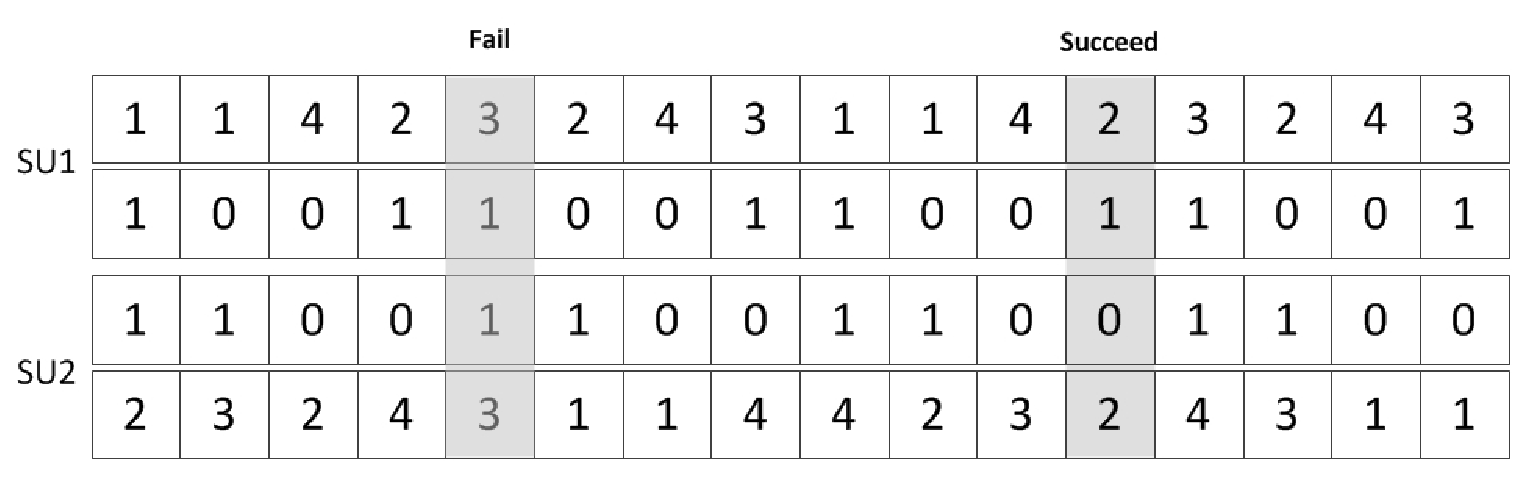
\includegraphics[width=9cm,height=3.5cm]{rend-basic.eps} 
        %\vspace{-0.4cm}
        \caption{An example of the basic link rendezvous scheme.} 
        \label{fig:rend-basic}
    \end{center} 
\end{figure} 

Based on \textbf{Algorithm \ref{al:rend1}}, we can get the following theorem:

\addtocounter{theorem}{-2}
\begin{theorem}
\label{th:exp_t}
The expectation of time slots to achieve a link rendezvous for \textbf{Algorithm \ref{al:rend1}}
is $E[T]=2T_e$, where $T_e$ is the expectation of the channel rendezvous time for a specific given channel hopping sequence.
\end{theorem}
\begin{proof}
According to the design of the transmission sequence of each SU, the probability that there is one sender and one receiver when two SUs hop to a common available channel is $0.5$, Therefore, if two SUs hop to a common available channel, the probability of a successful link rendezvous is $0.5$. If a link rendezvous fails because of that there is not a valid transmission pair, two SUs should continue the channel hopping process until a successful link rendezvous. Finally, the expectation of time slots to achieve a link rendezvous time is:
\begin{equation}
\sum_{i=1}^{\infty} T_e(1-0.5)^{(i-1)}(0.5) = \DF{T_e}{0.5} = 2T_e.
\end{equation}
\end{proof}
\subsection{Enhanced Link Rendezvous Scheme}
\label{sec:en_rend}
In the basic link rendezvous scheme, each SU should follow two sequences, the channel hopping sequence and the transmission sequence. In this section,  we propose an enhanced link rendezvous scheme that each SU can just follow a \textit{virtual channel hopping sequence} so each SU does not need to implement an existing channel hopping sequence and a transmission sequence simultaneously.\\

\vspace{-0.4cm}
Our basic idea is to combine the channel hopping sequence with the transmission sequence. Therefore, we expand the total $M$ practical channels to $2M$ \textit{virtual channels}.
For real channel $i$, we map it to two virtual channels $i$ and $i+M$. An example of generating the virtual channels when $M$ equals $4$ is shown in Fig. \ref{fig:virtual}. Therefore,
after this mapping process, for each SU, there are total $2M$ virtual channels.
Each SU hops according to a \textit{virtual channel hopping sequence} generated from the total $2M$ virtual channels. When a SU hops to the virtual channel $i$ that $i \leq M$, it should tune
its transceiver to the sending mode and hop to real channel $i$. On the other
side, when a SU hops to the virtual channel $i$ that $M<i\leq 2M$, it should tune its transceiver
to the receiving mode and  hop to real channel $i-M$. Furthermore, if channel
$i$ is available to a SU during current time slot, both  virtual channels $i$ and $i+M$
are also available to the SU.\\
\begin{figure}[hbtp] 
    \begin{center} 
        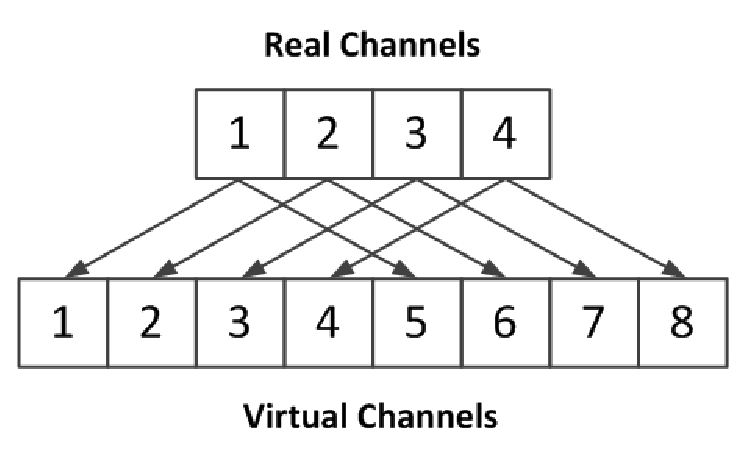
\includegraphics[width=6cm,height=3cm]{virtual.eps} 
        %\vspace{-0.4cm}
        \caption{An example of generating virtual channels.} 
        \label{fig:virtual}
    \end{center} 
\end{figure} 

Therefore, based on the virtual channel hopping sequence and 
the send-or-receive problem, a successful link rendezvous is defined as follows: %%%add a figure to show an example of virtual channel

\textit{Successful link rendezvous}: During time slot $t$, if the $i$th SU
hops to the virtual channel $c^{t}_i$ and the $j$th SU hops to the virtual channel
$c^{t}_j$, a successful link rendezvous is achieved if $|c^{t}_i-c^{t}_j|
= M$, $c^{t}_i\in \mathcal{C}^{t}_i$, and $c^{t}_j\in \mathcal{C}^{t}_j$,
where $\mathcal{C}^{t}_i$ and $\mathcal{C}^{t}_j$ are the current available
virtual channel sets of the $i$th and $j$th SU, respectively.\\

\vspace{-0.4cm}
According to the definition of a successful link rendezvous based on the virtual channel hopping sequence, it is quite different from a successful \textit{channel rendezvous} that two SUs hop to a common available channel at the same time slot. Therefore, all the existing channel hopping sequences which can guarantee a successful \textit{channel rendezvous} cannot achieve a successful \textit{link rendezvous}  based on the virtual channels.\\

\vspace{-0.4cm}
Our goal in this section is to design an efficient \textit{link rendezvous} scheme which
can achieve a fast successful link rendezvous between two SUs. The first step is to design a virtual channel hopping sequence based
on the total $2M$ virtual channels. The basic idea about the virtual channel hopping
sequence is to make each SU performs channel hopping according to the same
virtual channel hopping sequence $\mathcal{S}$ generated from $2M$ virtual channels. However,  since two SUs are fully distributed and
not synchronized, even though they follow the same virtual channel hopping sequence,
they may stay on the different positions of it. Therefore, the
sequence should try to achieve a successful link rendezvous regardless of different
positions of two SUs on the same virtual channel hopping sequence.\\

\vspace{-0.4cm}
The first step to generate such a virtual channel hopping sequence is to generate a basic
sequence $\mathcal{B}$ such that its length is $4M$ and $\mathcal{B}[i]=\mathcal{B}[j]
= j-i, 1\leq i<j\leq 4M$, for any $1\leq\mathcal{B}[i]\leq 2M$, where $\mathcal{B}[i]$ is
the $i$th element of $\mathcal{B}$. Therefore, each number in the range $[1,M]$
appears exactly twice in $\mathcal{B}$.


Based on the definition of $\mathcal{B}$, we can first get the following
lemma regarding the existence of $\mathcal{B}$.

\addtocounter{theorem}{1}
\begin{lemma}
\label{lemma:guar_rend1}
If two SUs follow the same basic virtual channel hopping sequence $\mathcal{B}$, the first SU starts from the $i$th element , the second SU
starts from the $j$th element, and $k=|i-j|>0$, they could both hop to 
 virtual channel $k$ if $k\leq 2M$, or virtual channel $4M-K$ if $2M<k<4M$, within $4M$ time slots.
\end{lemma}
\begin{proof}
According to the definition of $\mathcal{B}$, if $k\leq 2M$, there are two
elements in the sequence $\mathcal{B}[u]=\mathcal{B}[v]=k, v > u$, and $|v-u|=k$.
Therefore, the two SUs can all hop to the virtual channel $k$ within $4M$
time slots. If $2M<k\leq 4M$, since two SUs hop according to the same $\mathcal{B}$
circularly, the distance between them on the sequence is also $4M-K < 2M$.
Therefore, according to the definition of $\mathcal{B}$, there are two elements
in the sequence $\mathcal{B}[u]=\mathcal{B}[v]=4M-k, v > u$, and $|v-u|=4M-k$.\\
\end{proof}

Here is an example in Fig.\ref{fig:rend0}. In the example, we assume that $M=2$, SU1 starts from the first channel in $\mathcal{B}$, and  SU2 starts from the fourth channel in $\mathcal{B}$, during the fifth time slot, both SUs   hop to channel $3$. \\
\begin{figure}[hbtp] 
    \begin{center} 
        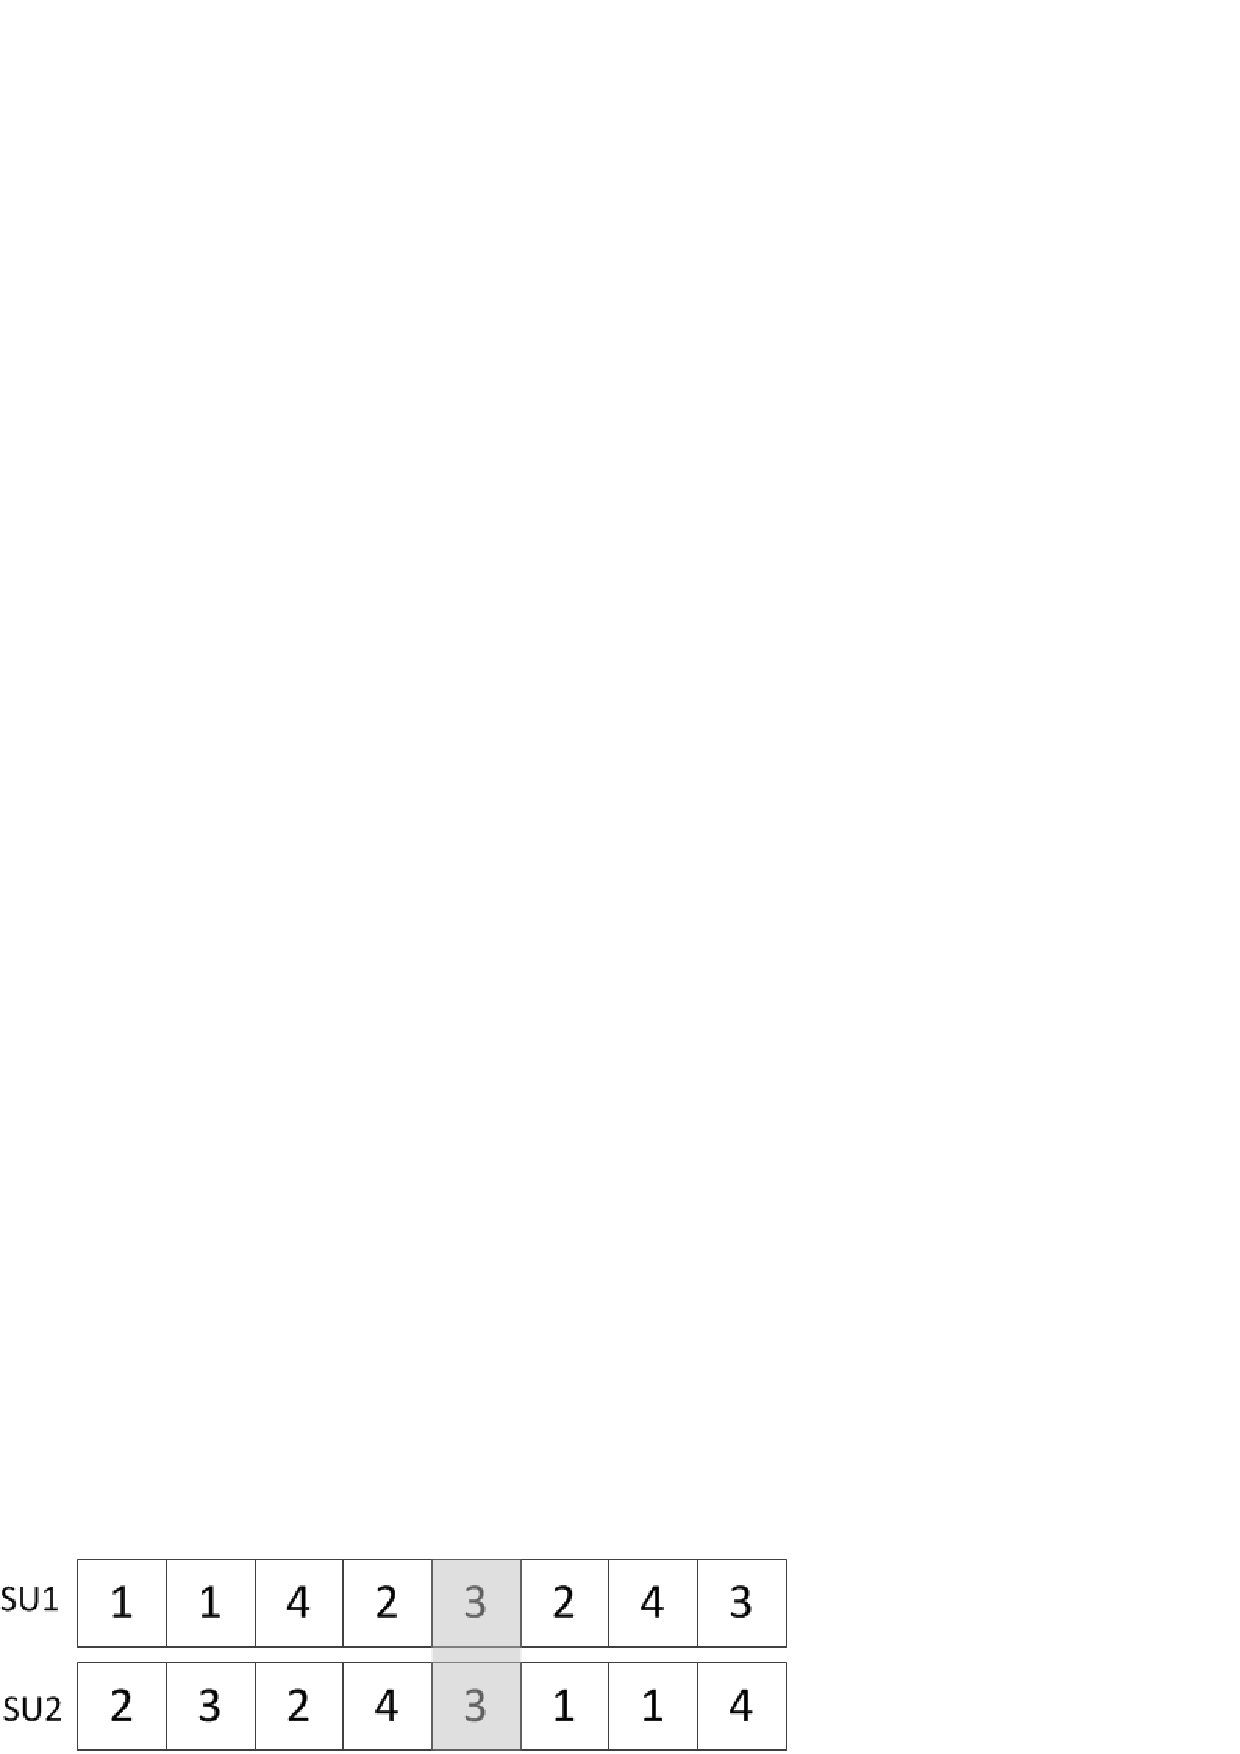
\includegraphics[width=8cm,height=2cm]{rend0.jpg} 
        %\vspace{-0.4cm}
        \caption{An example of the basic virtual channel hopping sequence.} 
        \label{fig:rend0}
    \end{center} 
\end{figure}

To get the final virtual channel hopping sequence $\mathcal{S}$, The second step
is to replace some elements in $\mathcal{B}$
according to the following manipulations: for each number $k$ that $\mathcal{B}[i]=\mathcal{B}[j]=k,
1\leq i<j\leq 4M$, if $k \leq M$, reset $\mathcal{B}[j] = k+M$, otherwise
reset $\mathcal{B}[j] = k-M$. An example is shown in Fig. \ref{fig:replace}, where $M=2$ and the basic sequence $\mathcal{B}$
could be $\{1,1,4,2,3,2,4,3\}$, after the replacements, the final channel
hopping sequence $\mathcal{S}$ should be $\{1,3,4,2,3,4,2,1\}$.\\
\begin{figure}[hbtp] 
    \begin{center} 
        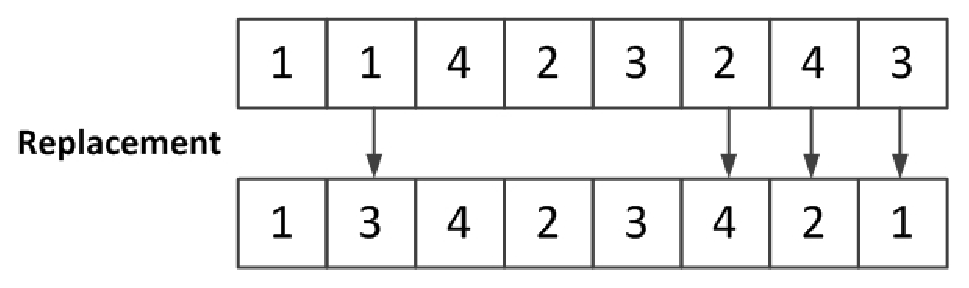
\includegraphics[width=8cm,height=2cm]{replace.eps} 
        %\vspace{-0.4cm}
        \caption{An example of the replacement manipulations.} 
        \label{fig:replace}
    \end{center} 
\end{figure}

In order to generate the virtual channel hopping sequence $\mathcal{S}$, we have the following lemmas about some important features of the basic virtual channel hopping sequence $\mathcal{B}.$

\begin{lemma}
\label{lemma:noexist}
When $2M\ mod\ 4=2$, $\mathcal{B}$ does not exist.
\end{lemma}
\begin{proof}
According to the definition of $\mathcal{B}$, designing the basic
sequence is equivalent to dividing all the indexes $1,2,\dots, 4M$, these $4M$ numbers into
two lists $\mathcal{L}_{1}$ and $\mathcal{L}_{2}$, each of which has exactly
$2M$ different numbers, such that for $k=1,2,\dots,2M$, $\mathcal{L}_{2}[k]
- \mathcal{L}_{1}[k] = k$. Then, we have
        \begin{equation}
        \label{eq:sum1}
        \sum^{2M}_{k=1}\mathcal{L}_{2}[k]-\sum^{2M}_{k=1}\mathcal{L}_{1}[k]=\sum^{2M}_{k=1}k=\DF{2M(2M+1)}{2},
        \end{equation}
        \begin{equation}
        \label{eq:sum2}
        \sum^{2M}_{k=1}\mathcal{L}_{2}[k]+\sum^{2M}_{k=1}\mathcal{L}_{1}[k]=\sum^{4M}_{k=1}k=2M(4M+1).
        \end{equation}
        Combining \eqref{eq:sum1} and \eqref{eq:sum2}, we can get 
        \begin{equation}
        \label{eq:sum3}
        \sum^{2M}_{k=1}\mathcal{L}_{2}[k]=\DF{10M^{2}+3M}{2}.
        \end{equation}
        When $2M\ mod\ 4=2$, $M$ is an odd number that can be represented as $M=2e+1, e\geq 0$, thus
        \begin{equation}
        \label{eq:sum4}
        \sum^{2M}_{k=1}\mathcal{L}_{2}[k]=\DF{10(2e+1)^{2}+3(2e+1)}{2}=20e^2+23e+\DF{13}{2}.
        \end{equation}
        
 the right-hand side of \eqref{eq:sum4} is not an integer which contradicts the fact that it is a sum of $4M$ integers.
\end{proof}
     
\begin{lemma}
\label{lemma:exist}
When $M>1$ and $2M\ mod\ 4=0$, $\mathcal{B}$ exists.
\end{lemma}
\begin{proof}
        When $M=2$, sequence $\{1,1,4,2,3,2,4,3\}$ satisfies the requirements
of our desired basic link rendezvous sequence.
        When $M>2$, the proof can be found in the second page of \cite{tSkolem57OCDOI}.
\end{proof}

Based on the proof of \textbf{ Lemma \ref{lemma:noexist}} and \textbf{ Lemma
\ref{lemma:exist}}, we propose \textbf{Algorithm \ref{al:generate}} to generate
our virtual channel sequence $\mathcal{S}$.

\begin{algorithm} 
  \caption{The algorithm for generating the virtual channel hopping sequence}
  \begin{algorithmic}[1] 
  \label{al:generate}
    \REQUIRE ~~\\
    The number of channels : $M$
    \ENSURE ~~\\
    The desired rendezvous sequence: $\mathcal{S}$\\
    \STATE $n = 2M$;
    \IF{$n\%4==2$}
        \STATE $n = n+2$;
    \ENDIF
    \IF{$n==4$}
         \STATE $\mathcal{S}=\{1,1,4,2,3,2,4,3\}$;
    \ELSE
        \STATE Initialize $\mathcal{S}$ as a list of length $4n$;
        \STATE Let $P$ be an empty list;
        \STATE $m=\lfloor n/4 \rfloor$;
        \STATE Add all pairs $(4m+r, 8m-r)$, for $r=0,1,\dots,2m-1$, to $P$;
        \STATE Add pairs $(2m+1, 6m)$ and $(2m, 4m-1)$ to $P$;
        \STATE Add all pairs $(r, 4m-1-r)$, for $r=1,3,\dots,m-1$, to $P$;
        \STATE Add pair $(m, m+1)$ to $P$;
        \STATE Add all pairs $(m+2+r, 3m-1-r)$, for $r=0,1,\dots,m-3$, to $P$;
    \FOR{$i=1$ to $n$}
        \STATE $\mathcal{S}[P[i].first] = \mathcal{S}[P[i].second] = P[i].second
- P[i].first$;
    \ENDFOR
    \ENDIF
    \FOR{$i=1$ to $2n$}
        \IF{$\mathcal{S}[i] > 2M$}
             \STATE $\mathcal{S}[i]\ \% = 2M$; //limit each value to $[1,2M]$
        \ENDIF
    \ENDFOR
    \FOR{$i=1$ to $2n$}
        \STATE //replacement manipulations
        \IF{this the second time that $k=\mathcal{S}[i]$ appears}
             \IF{$k \leq M$}
                  \STATE $\mathcal{S}[i] = \mathcal{S}[i] + M;$
             \ENDIF
             \IF{$k > M$}
                  \STATE $\mathcal{S}[i] = \mathcal{S}[i] - M;$
             \ENDIF
        \ENDIF
    \ENDFOR
    \RETURN $\mathcal{S}$;
  \end{algorithmic}
\end{algorithm} 

According to \textbf{Algorithm \ref{al:generate}}, if $M>0$ and $2M\ mod\ 4=2$, the length of $\mathcal{S}$ should be larger than $4M$ in order to
guarantee the existence of $\mathcal{S}$. Furthermore, we have the following
lemma about $\mathcal{S}$ regarding a successful link rendezvous. After getting
the virtual channel hopping sequence $\mathcal{S}$, we can get the
following lemma regarding a  successful link rendezvous:

\begin{lemma}
\label{lemma:guar_rend2}
Assume that when a link rendezvous process begins, the first SU is on $i$th element of
$\mathcal{S}$, the second SU is on the $j$th element of $\mathcal{S}$, and
$k=|i-j|>0$. Within $4M$ time slots, two SUs can hop to two different virtual
channels
$c_1$ and $c_2$ such that $|c_1-c_2|=M$. 
\end{lemma}
\begin{proof}
According to \textbf{Lemma \ref{lemma:guar_rend1}}, within $4M$ time slots,
two SUs can hop to the same virtual channel $c$ on the different positions
of $\mathcal{B}$. Since we perform the replacement manipulations of $\mathcal{B}$
to get $\mathcal{S}$,  the manipulation can make the same two $c$ values
in $\mathcal{B}$ change to two different values $c_1$ and $c_2$ such that
$|c_1-c_2|=M$. Therefore, within $4M$ time slots,  two SUs can hop to two
different virtual channels $c_1$ and $c_2$ such that $|c_1-c_2|=M$.
\end{proof}

\vspace{-0.1cm}
An example of Lemma \ref{lemma:guar_rend2} is shown in Fig. \ref{fig:rend1}, where $M = 2$, the virtual channel sequence is $\{1, 3, 4, 2, 3, 4, 2, 1\}$, SU1 starts from the first element, and SU2 starts from the third element. Within $4M = 8$ time slots, two SUs first hop to channel $2$ and $4$ that $4-2 = 2 = M$ during the fourth time slot, and then hop to channel $1$ and $3$ that $3-1 = 2 = M$ during the eighth time slot.\\
\begin{figure}[hbtp] 
    \begin{center} 
        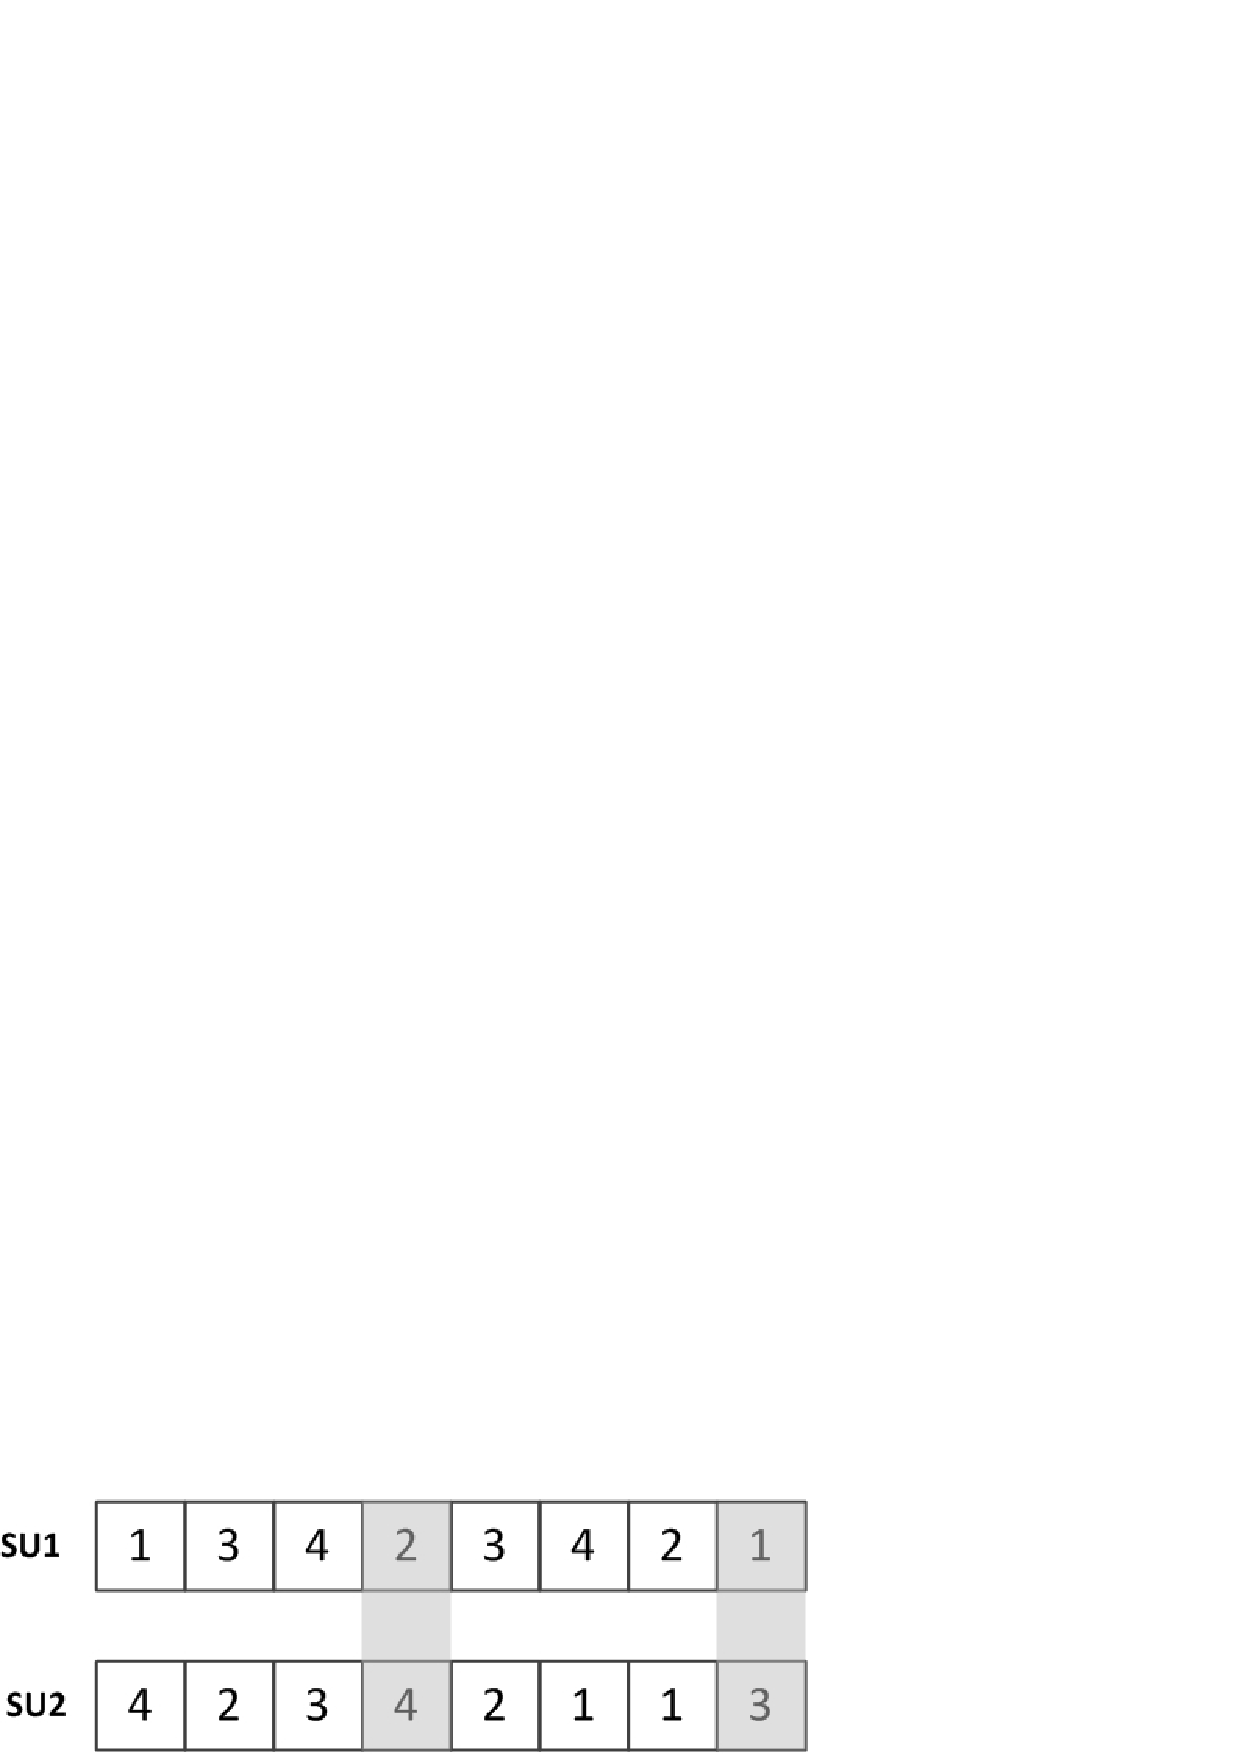
\includegraphics[width=8cm,height=2.2cm]{rend1.jpg} 
        %\vspace{-0.4cm}
        \caption{An example of the virtual channel hopping sequence.} 
        \label{fig:rend1}
    \end{center} 
\end{figure}

Since a necessary condition for a successful link rendezvous is that two SUs
should hop to two virtual channels $c_1$ and $c_2$, respectively, such that
$c_1>c_2, c_1-c_2=M$, we can design a channel hopping scheme based on \textbf{Lemma 6}. However, the problem is that if the virtual channel $c_2$
is not a common available virtual channel, the two SUs still cannot achieve
a successful rendezvous, even if they hop to $c_1$ and $c_2$
during the same time slot. Therefore, after every $4M$ time slots, if two SUs did
not achieve a successful link rendezvous, each SU should restart a new virtual channel
hopping process from a new starting element in $\mathcal{S}$ to make the two SUs
can hop to new virtual channels $c^{'}_1$ and $c^{'}_2$, respectively, until $c^{'}_2$ is a common available virtual channel. Therefore,
we design the following distributed link rendezvous scheme  for each SU in \textbf{Algorithm \ref{al:rend2}}:
\begin{algorithm} 
  \caption{The distribute link rendezvous algorithm for each SU}
  \begin{algorithmic}[1] 
  \label{al:rend2}
    \REQUIRE ~~\\
    The total number of channels: $M$\\

    \STATE Generate the virtual channel hopping sequence $\mathcal{S}$;
    \STATE Randomly choose a starting index $i$ on $\mathcal{S}$;
    \STATE $count=0$;// count time slots
    \WHILE{Not rendezvous}
         \IF{$\mathcal{S}[i] > M$ and $\mathcal{S}[i]$ is currently available}
            \STATE Hop to channel $\mathcal{S}[i]-M$ and tune to the receiving
mode;
         \ENDIF
         \IF{$\mathcal{S}[i] \leq M$  and $\mathcal{S}[i]$ is currently available}
            \STATE Hop to channel $\mathcal{S}[i]$, tune to the sending
mode,
and send RTS packets on the channel;        \ENDIF
         \STATE count++;
         \IF{$count >= 4M$}
            \STATE $count = 0$;
            \STATE Randomly generate a new $i$;//reset $i$
         \ELSE
            \STATE $i++$;
            \IF{$i>4M$}
                \STATE $i = 1$;//circular hop
            \ENDIF
         \ENDIF
    \ENDWHILE
  \end{algorithmic}
\end{algorithm}  

Based on \textbf{Algorithm\ref{al:rend2}}, we can get the following lemma:
\begin{lemma}
The probability that two SUs fail to rendezvous within every $4M$ time slots
is $p_f\approx 1-p_c$, where $p_c$ is the probability that a channel is a
common available channel of the two SUs. 
\end{lemma}
\begin{proof}
The probability that two SUs choose different starting indexes in $\mathcal{S}$
is $\DF{4M(4M-1)}{(4M)^2}=\DF{4M-1}{4M}$. Two SUs can achieve a  successful
link rendezvous only when they choose different starting indexes and the virtual 
channel they will hop to is available to both of them. Therefore, the probability
that two SUs achieve a successful rendezvous during every $4M$ time slots
is $\DF{4M-1}{4M}p_c$. Finally, the fail probability is $1-\DF{4M-1}{4M}p_c=\DF{4M-4Mp_c-p_c}{4M}=\
1-p_c-\DF{p_c}{4M}\approx 1-p_c$
\end{proof}

Finally, we can get the \textbf{Theorem 2} regarding the average link rendezvous time of the enhanced link rendezvous scheme in \textbf{Algorithm\ref{al:rend2}}.\addtocounter{theorem}{-6}
\begin{theorem}
\label{th:exp_t}
The expectation of link rendezvous time slots for \textbf{Algorithm\ref{al:rend2}}
is $E[T]=\DF{4M}{p_c}$, where $M$ is the total number of channels and $p_c$
is the probability that a channel is a common available channel of the two
SUs.
\end{theorem}
\begin{proof}
The expectation of link rendezvous time slots is:
\begin{equation}
\sum_{i=1}^{\infty} 4Mp_{f}^{(i-1)}(1-p_f) = \DF{4M}{1-p_f} = \DF{4M}{p_c}.
\end{equation}
\end{proof}

\section{Rendezvous with Directional Antenna}
\subsection{System Model and Problem Description}
\label{sec:des}
In this paper, we consider two SUs, coexisting with several PUs, who want to rendezvous with each other. Each SU can opportunistically access a total of $M$ channels. Each SU is equipped with a directional antenna that can transmit or receive signals on a transmission sector with a certain angle. We assume that the directional antenna of each SU can adjust the angle of a transmission sector. The two considered SUs are located within the transmission range of each other, and they can implement the same channel rendezvous scheme which can guarantee a successful channel rendezvous within a bounded time.\\

\vspace{-0.6cm}
The transmission area of a SU is evenly divided into $N$ sectors without overlaps. We assume that during each time slot, a SU can only transmit in one sector and on one channel. The index of each transmission sector does not change after the initialization.  When two SUs with directional antennas try to set up a communication link between them, they should tune their antennas to specific directions so that their current transmission sectors can cover each other, which is called a successful \textit{sector rendezvous}. If the SU receiver is located in the $p$th transmission sector of the SU sender and the SU sender is located in the $q$th transmission sector of the SU sender, we denote $(p,q)$ as a \textit{sector rendezvous pair}. We get the following theorem about the sector rendezvous and sector rendezvous pair.% in Fig. 2 show one is they covered each other, one is not
\begin{theorem}
\label{th:exist}
There always exists a sector rendezvous between two SUs and the rendezvous pair is unique, regardless of the number of transmission sectors of each SU.
\vspace{-0.4cm}
\end{theorem}
\begin{proof}
We assume that the SU receiver is covered by the $p$th transmission sector of the SU sender and the SU sender is covered by the $q$th transmission sector of the SU receiver. Since each sector of a SU does not overlap with another sector, both $p$ and $q$ are unique (if a SU is located on the border of a transmission sector, only one sector is  counted). Therefore, when the SU sender is on the transmission sector $p$ and the SU receiver is on transmission sector $q$ simultaneously, they achieve a successful sector rendezvous. Since $p$ and $q$ are unique, the sector rendezvous pair $(p, q)$ is also unique.
\end{proof}

\vspace{-0.2cm}After tuning its directional antenna to each transmission sector, a SU performs a predetermined channel rendezvous scheme which can guarantee a successful channel rendezvous within the maximum time to rendezvous (\textit{MTTR}). If the SU does not rendezvous with another SU within \textit{MTTR} time slots in the current transmission sector, it hops to the next transmission sector and repeats the channel rendezvous process. Therefore, in this paper, we only consider how to let two SUs achieve a successful sector rendezvous, given  a specific channel rendezvous scheme that can guarantee a successful channel rendezvous.\\

\vspace{-0.6cm}
We define the process that a SU hops to a transmission sector as the \textit{sector hopping process}. If we denote the index of the sector a SU is on at time slot $t$ as $S_{t}$, the sequence $S_{0}, S_{1}, \dots, S_{t}, \dots$ is called a \textit{sector hopping sequence}. An example in Fig. \ref{fig:necessary} shows why both SUs should perform the sector hopping process by following a sector hopping sequence. If the SU receiver just stays within a sector waiting for the RTS packet, it may never hear the SU sender since their transmission sectors may never cover each other like the scenario in Fig. \ref{fig:necessary}. Since a SU does not know others' location before a successful blind rendezvous, both SUs should perform the sector hopping process to achieve a successful sector rendezvous.\\
 \begin{figure}[hbtp] 
    \begin{center} 
        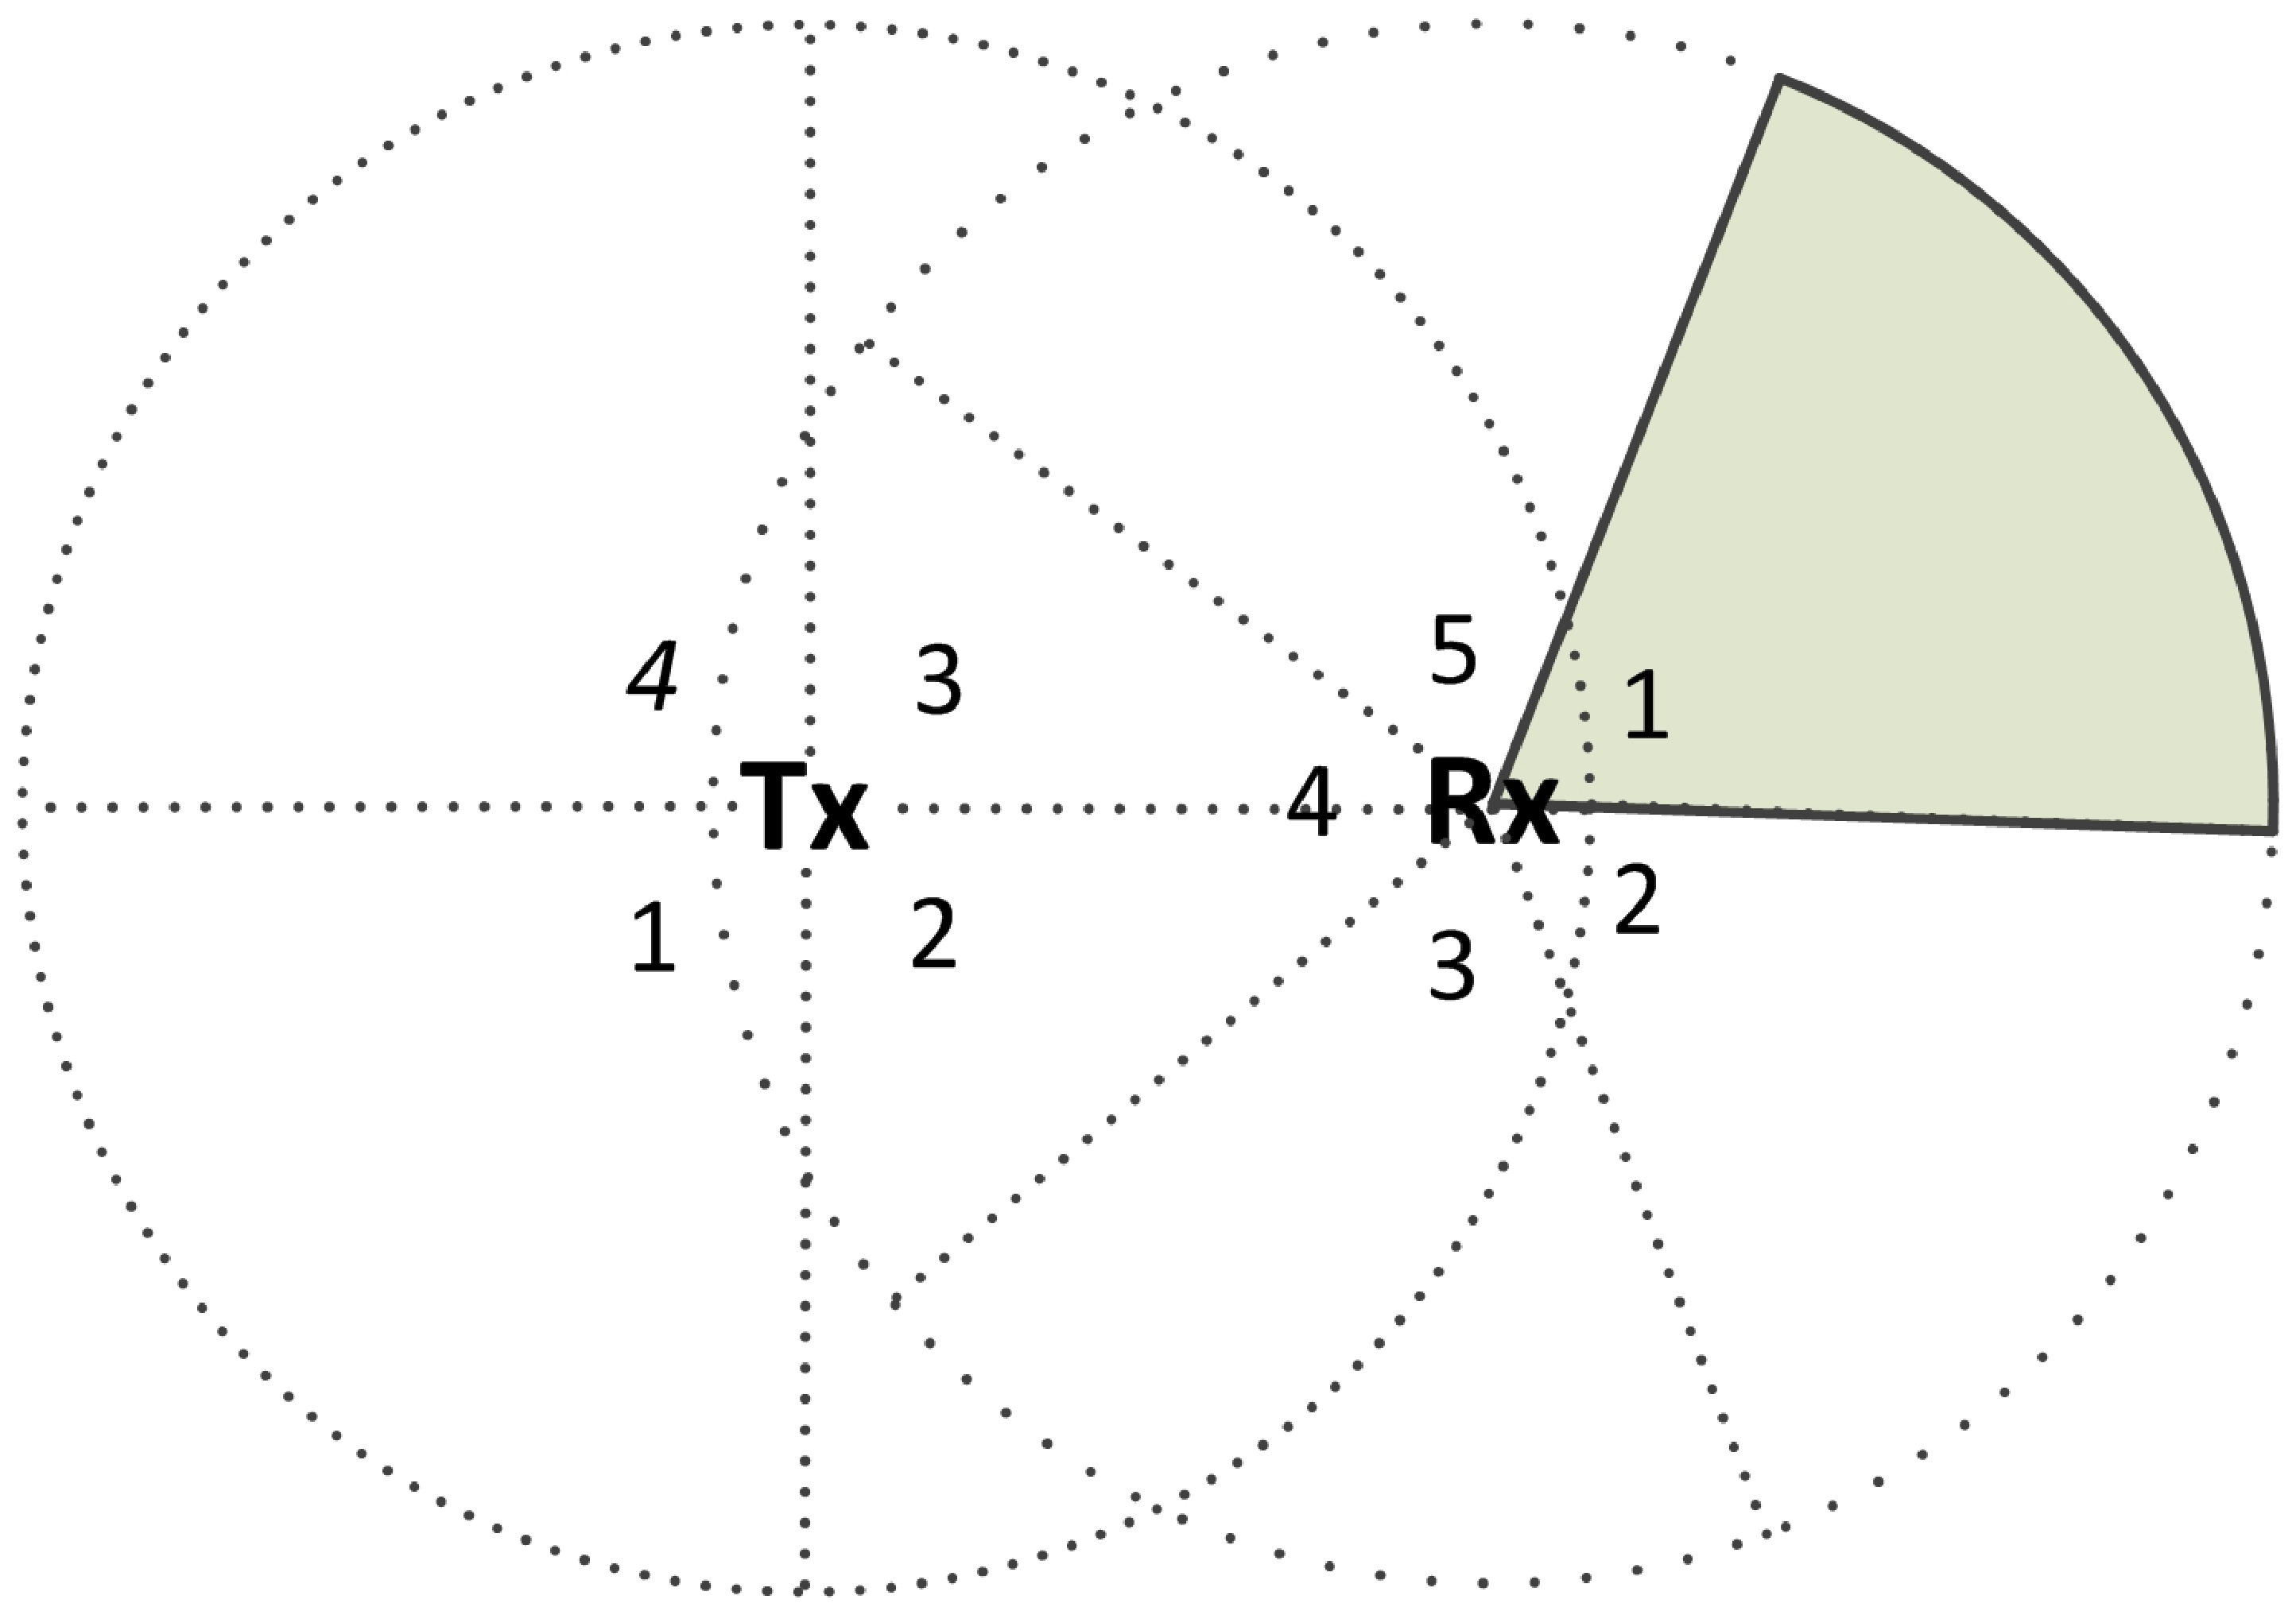
\includegraphics[width=5cm,height=3.5cm]{need.eps} 
         \vspace{-0.2cm}
        \caption{An example to show the necessity of the sector hopping process.} 
        \label{fig:necessary}
    \end{center} 
\end{figure}
 
\vspace{-0.6cm}
The \textit{sector rendezvous problem} is defined as follows. We denote the sector hopping sequences of the SU sender and receiver as $S_{t_{0}}^{s}, S_{t_{1}}^{s}, \dots , S_{t_{t}}^{s}$ and $S_{t_{0}}^{r}, S_{t_{1}}^{r}, \dots , S_{t_{t}}^{r}$, respectively, where $t_{0}$ is the time the SU sender starts the rendezvous process by sending a RTS packet. Two SUs may not start the sector rendezvous process simultaneously under the blind information scenario.  We assume that the rendezvous pair of the two SUs is $(p,q)$ and they achieve sector rendezvous at time $t_{t}$ if  $S_{t_{t}}^{s} = p,  S_{t_{t}}^{r} = q$. Our goal is to design a distributed sector hopping sequence for each SU that can guarantee a successful sector rendezvous and the time for the rendezvous $t_{t}-t_{0}$ is bounded.\\

\vspace{-0.6cm}
The first problem about the sector rendezvous problem is the \textit{indexing problem}. As two SUs do not know any information about each other before a successful channel rendezvous, the way they index their sectors may be quit different and unknown to each other, which may lead to $p\neq q$ for a rendezvous pair. Fig. \ref{fig:index} shows an example of the indexing problem, in which the rendezvous pair is $(2, 4)$. We denote the number of the sectors of the SU sender and SU receiver as $N_{s}$ and $N_{r}$, respectively. We can notice that the indexes of all the sectors of a SU form a permutation of the numbers from $1$ to $N_{s}$ or $N_{r}$. Our goal is to design a distributed sector hopping sequence for each SU which can guarantee a successful sector rendezvous within a bounded time considering the indexing problem.\\
\begin{figure}[hbtp] 
    \begin{center} 
        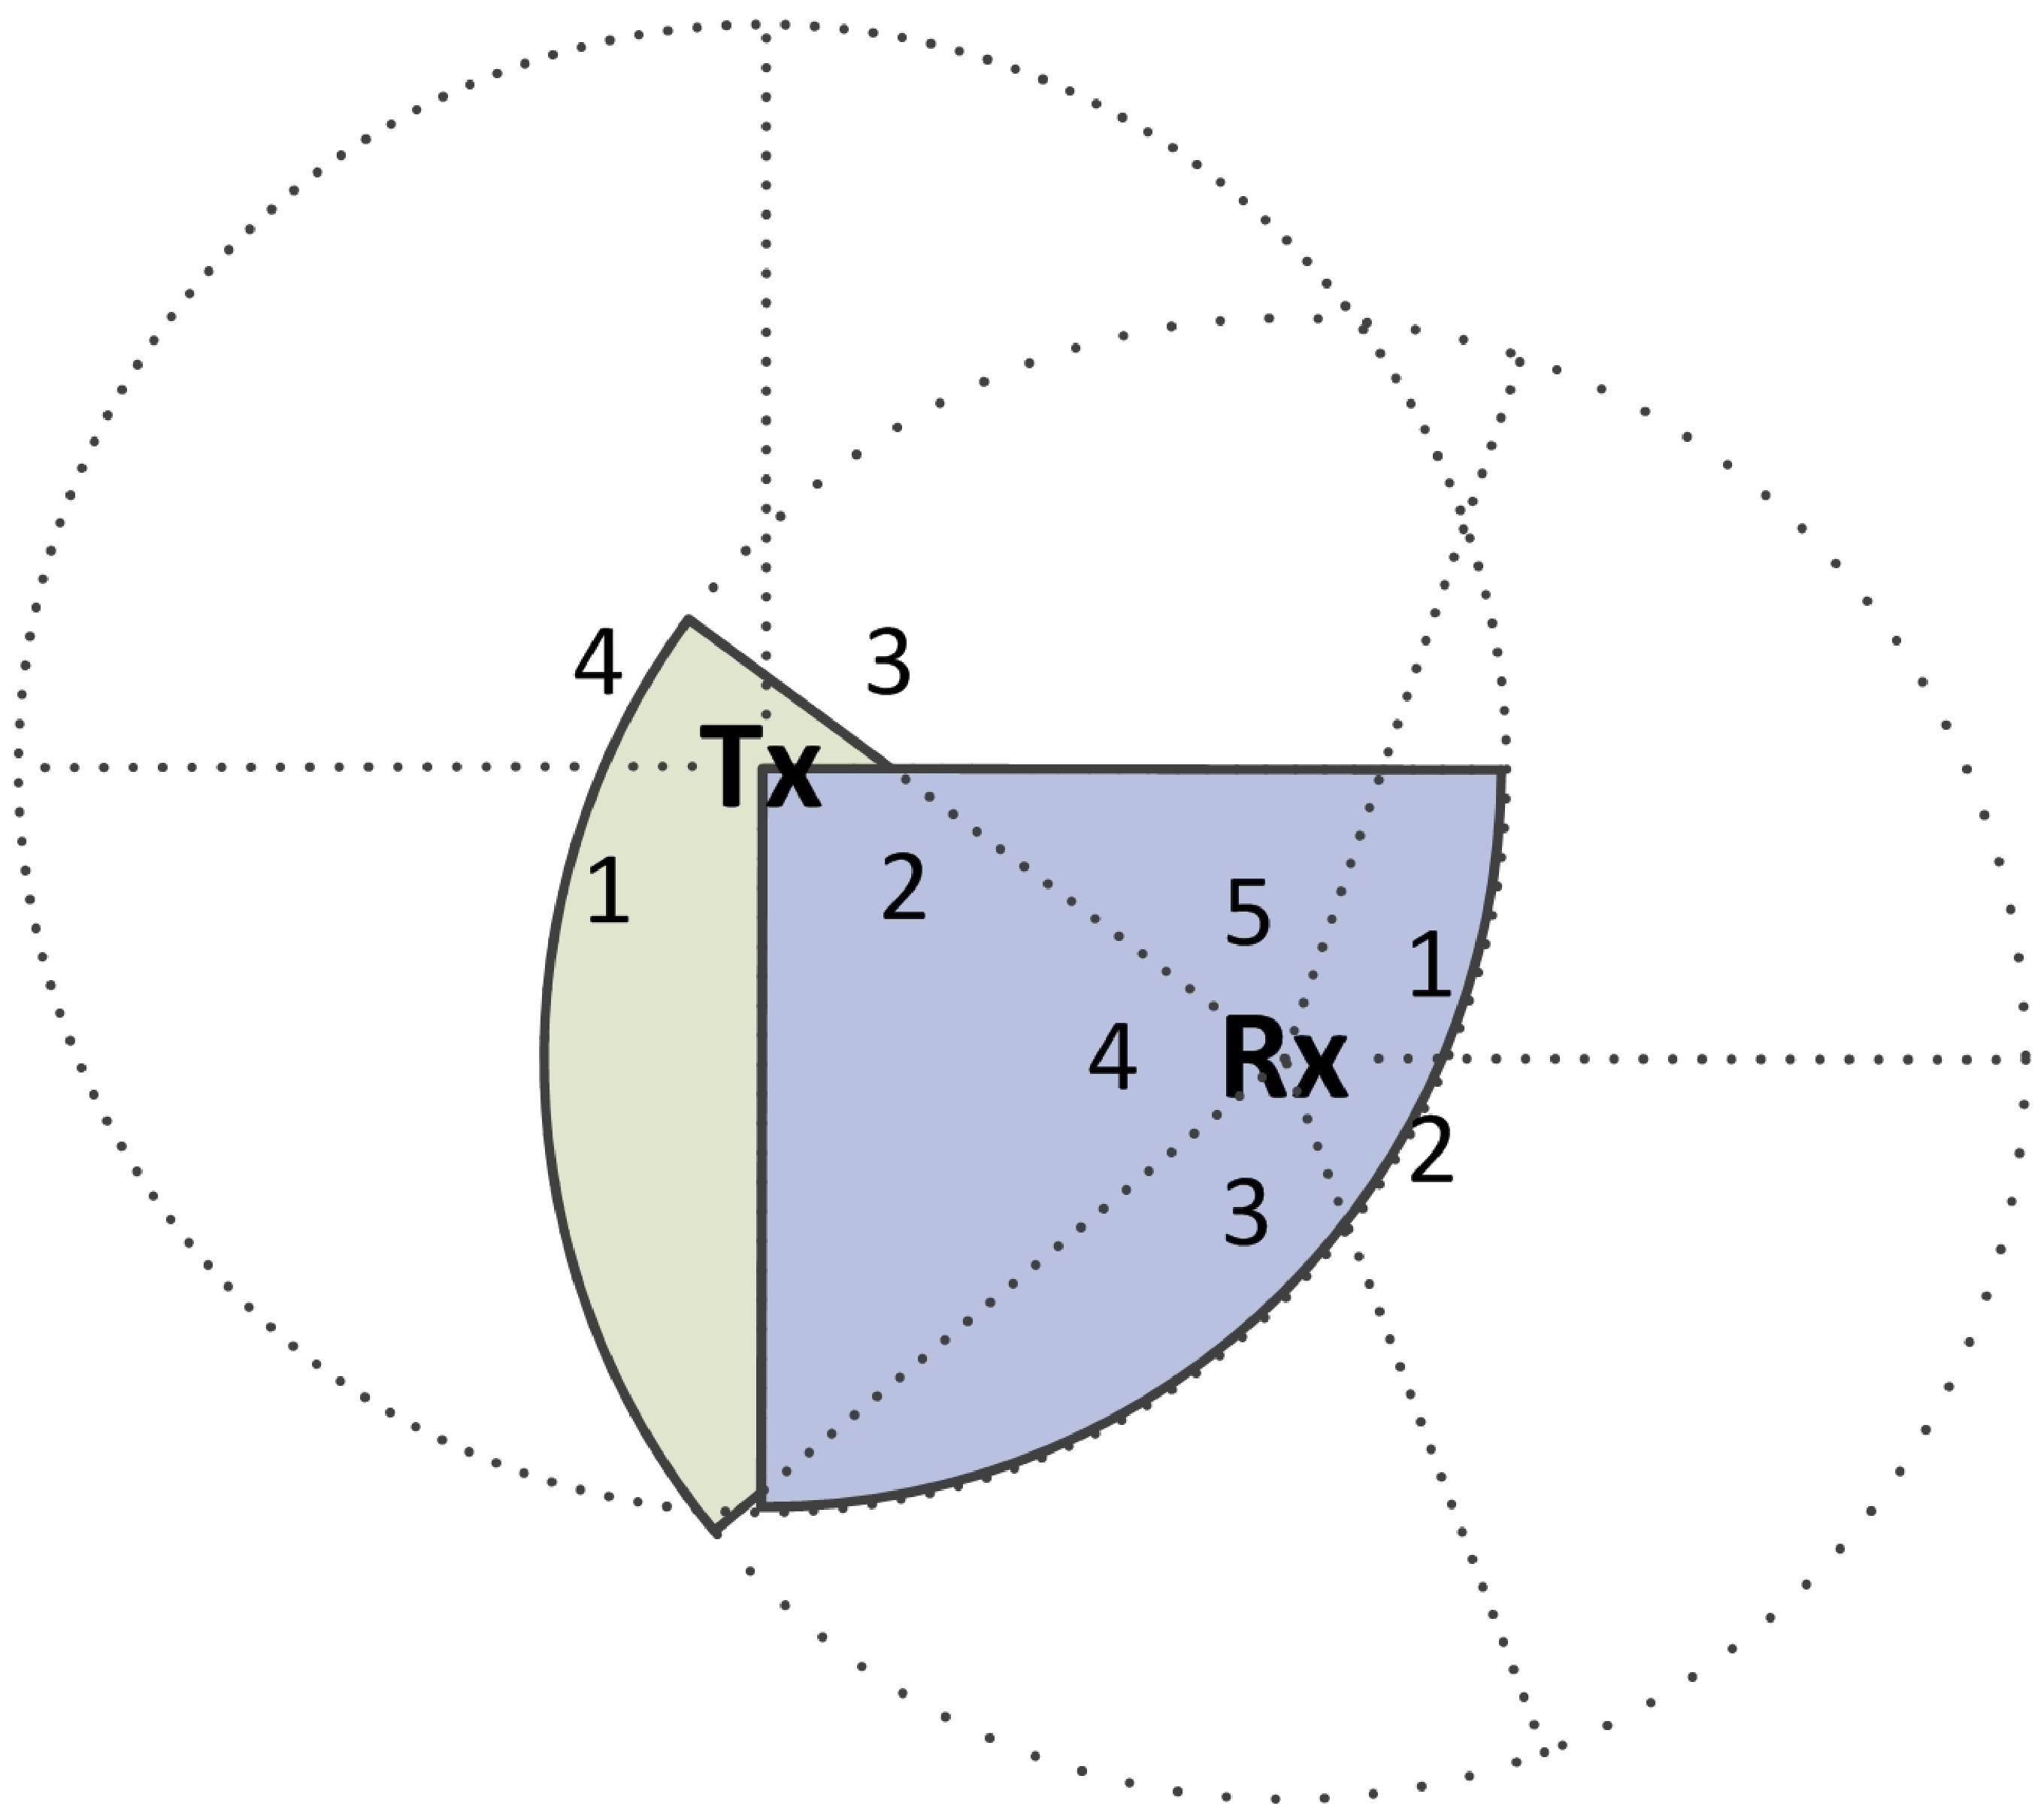
\includegraphics[width=4cm,height=3.5cm]{index.eps} 
         \vspace{-0.2cm}
        \caption{An example of the indexing problem and different sector number problem.} 
        \label{fig:index}
    \end{center} 
\end{figure}

\vspace{-0.6cm}
The second problem is called the \textit{different sector number problem} which means that the number of sectors of each SU may be different and each SU does not know the number of sectors of the other SU before exchanging information. This is a very practical issue when two SUs' transmission parameters are different due to hardware constrains or surrounding environments. Therefore, the optimal transmission angle of each SU's  directional antenna may be different. Especially, when two SUs do not know any information about each other during a blind rendezvous process, how can they configure the same transmission parameters for their antennas? An example is shown in Fig. \ref{fig:index}, where $N_{s} = 4$ and $N_{r} = 5$. Under this scenario, our goal is to design a distributed sector hopping sequence for each SU which can guarantee a successful sector rendezvous within a bounded time, regardless of different sector indexes and different total number of sectors.\\

\vspace{-0.6cm}
In the following sections, we propose distributed schemes that can guarantee a successful sector rendezvous considering both the indexing problem and different sector number problem.
\vspace{-0.2cm}
\subsection{Rendezvous Scheme Considering the Same Number of Sectors}
\label{sec:equal}
We first propose a sector rendezvous scheme considering the same number of sectors and the indexing problem. This may not be a general scenario. However, this scheme is a basis for the scheme considering the general scenario.\\

\vspace{-0.6cm}
Under this scenario, we denote the number of sectors for the SU sender and SU receiver as $N_{s} = N_{r} = N$ and the rendezvous sector pair is $(p, q)$, where $1\leq p,q \leq N$. According to the indexing problem, $(p, q)$ could be any element from $\{1, 2, \dots, N\} \times \{1, 2, \dots, N\}$, where $\times$ is the Cartesian product of the two sets. Our goal is to design a sector rendezvous scheme which can guarantee a successful sector rendezvous under this scenario.\\

\vspace{-0.6cm}
In our proposed scheme, the SU receiver always hops circularly according to the sector hopping sequence which is a circularly left shift of the sequence $1, 2, \dots, N$. The shift is based on the starting index. The SU receiver can start sector hopping from any sector index. For instance, when $N = 5$, the sector hopping sequence is $3, 4, 5, 1, 2, 3, 4, 5, 1, 2, \dots$ if it starts from sector $3$ based on its indexing method.  The SU sender performs the same way as the SU receiver but increasing the starting index by $1$ after each round. For example, when $N = 5$, the sector hopping sequence for the SU sender will be $4, 5, 1, 2, 3, 5, 1, 2, 3, 4, \dots$, if it starts from sector $4$ based on the SU sender's indexing method. If the rendezvous pair is $(1, 4)$, two SUs can achieve a sector rendezvous after $6$ times of sector hopping. Fig. \ref{fig:example1} shows an example of a successful sector rendezvous under the same sector number. The distributed algorithms for the SU receiver and SU sender to generate the sector hopping sequence are shown in \textbf{Algorithm \ref{al:seq_rev}} and \textbf{Algorithm \ref{al:seq_send}}, respectively.
\begin{figure}[hbtp] 
    \begin{center} 
        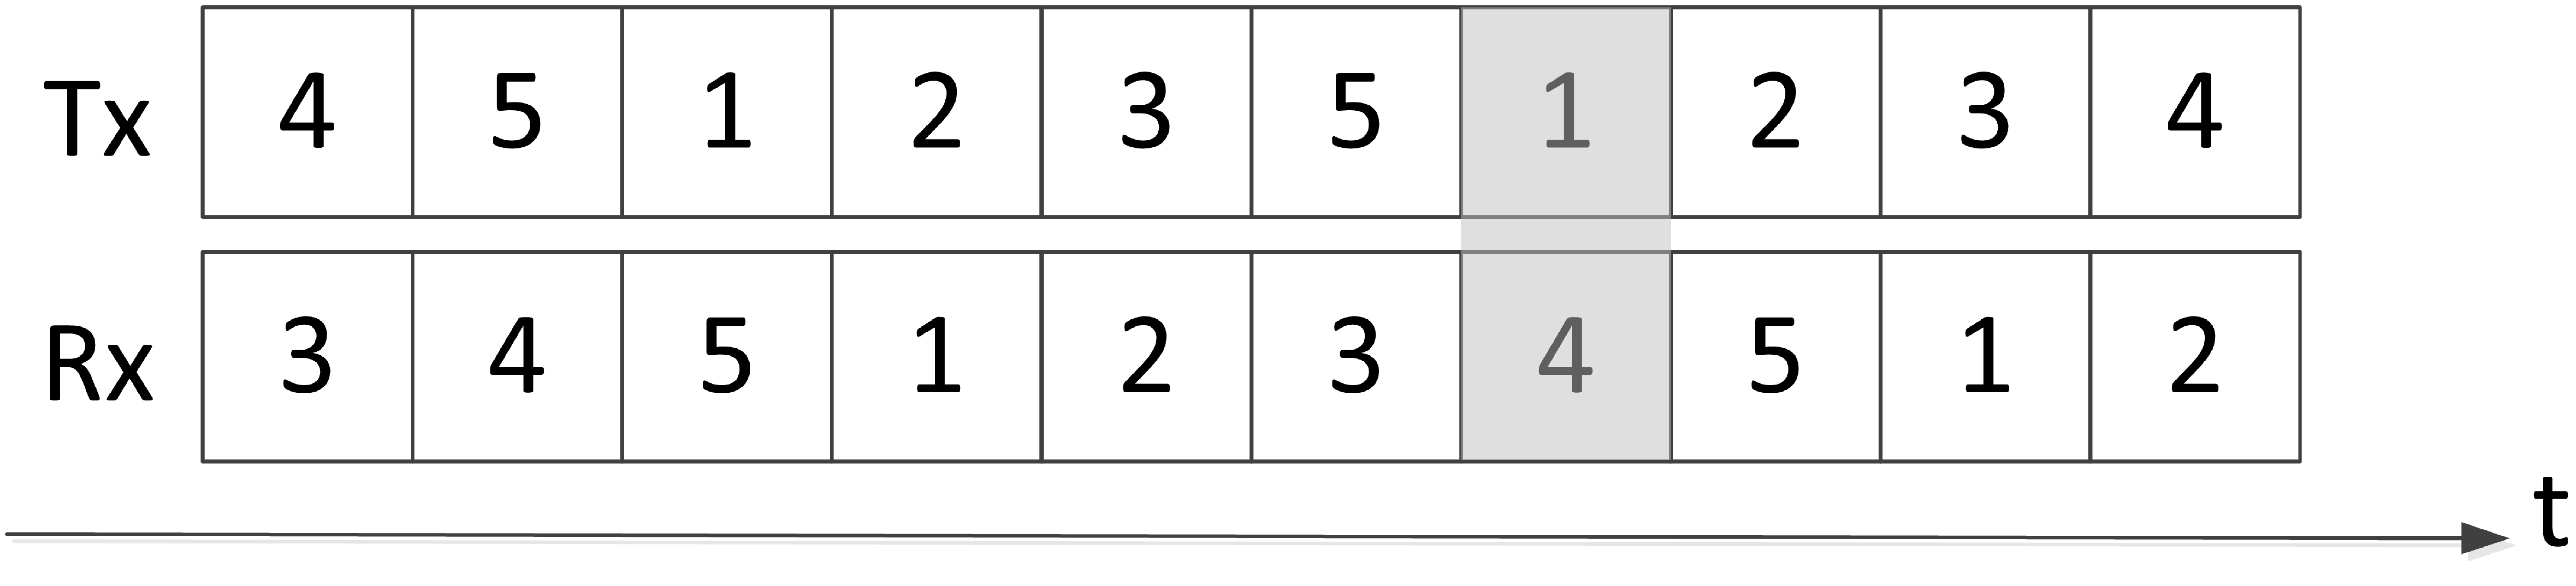
\includegraphics[width=8cm,height=2cm]{seq1.eps} 
         \vspace{-0.2cm}
        \caption{An example of a sector rendezvous under the same sector number.} 
        \label{fig:example1}
    \end{center} 
\end{figure}

\begin{algorithm} 
  \caption{Generate the sector hopping sequence for the SU receiver under the same sector number}
  \begin{algorithmic}[1] 
  \label{al:seq_rev}
    \REQUIRE ~~\\
    The number of sectors: $N$\\
    Current index of sector: $\theta_{i}$\\
    \ENSURE ~~\\
    The index of the next sector: $\theta_{i+1}$\\
    \IF{$\theta_{i}$ is null}
        \STATE // this is the first index
        \STATE $\theta_{i+1} = $ a random number from $[1, N]$;
    \ELSE
        \STATE $\theta_{i+1} = \theta_{i} + 1$;
        \IF{$\theta_{i+1} > N$}
                \STATE $\theta_{i+1} = 1$;
        \ENDIF
    \ENDIF
    \RETURN{$\theta_{i+1}$}
  \end{algorithmic} 
\end{algorithm}
\begin{algorithm} 
  \caption{Generate the sector hopping sequence for the SU sender under the same sector number}
  \begin{algorithmic}[1] 
  \label{al:seq_send}
    \REQUIRE ~~\\
    The number of sectors: $N$\\
    Current index of sector: $\theta_{i}$\\
    Starting index of current round: $\theta_{s}$\\
    \ENSURE ~~\\
    The index of the next sector: $\theta_{i+1}$\\
    \IF{$\theta_{i}$ is null}
        \STATE // this is the first index
        \STATE $\theta_{i+1} = $ a random number from $[1, N]$;
        \STATE $\theta_{s} = \theta_{i+1}$; // update $\theta_{s}$
    \ELSE
                \STATE $\theta_{i+1} = \theta_{i} + 1$;
        \IF{$\theta_{i+1} > N$}
                \STATE $\theta_{i+1} = 1$;
        \ENDIF
        \IF{$\theta_{i+1} == \theta_{s}$}
                \STATE $\theta_{s} = \theta_{s} + 1$; // update $\theta_{s}$
                \IF{$\theta_{s} > N$}
                        \STATE $\theta_{s} = 1$;
                \ENDIF
                \STATE $\theta_{i+1} = \theta_{s}$; // start a new round
        \ENDIF
    \ENDIF
    \RETURN{$\theta_{i+1}$}
  \end{algorithmic} 
\end{algorithm}

Based on \textbf{Algorithm \ref{al:seq_rev}} and \textbf{Algorithm \ref{al:seq_send}}, we can get \textbf{Theorem \ref{th:guarantee1}}.
\begin{theorem}
\label{th:guarantee1}
By following the sector hopping sequences generated by  \textbf{Algorithm \ref{al:seq_rev}} and \textbf{Algorithm \ref{al:seq_send}}, two SUs can achieve a successful sector rendezvous within $N^{2}$ sector hops. The average sector hops for a successful sector rendezvous is $N^{2}/2$.
\vspace{-0.2cm}
\end{theorem}
\begin{proof}
Assume that the sector rendezvous pair is $(p, q)\in \{1, 2, \dots, N\} \times \{1, 2, \dots, N\}$, where $\times$ is the Cartesian product of the two sets, and during the first round, when the SU sender is on its $p$th sector, the SU receiver is on its $\beta_{1} = \beta_{0}\%N+1$ sector, where $1\leq \beta_{0} \leq N$. According to \textbf{Algorithm \ref{al:seq_send}}, during the next $N-1$ rounds, when the SU sender is on its $p$th sector, the SU receiver should be on sectors $\beta_{2} = (\beta_{0}-1+N)\%N+1, \beta_{3} = (\beta_{0}-2+N)\%N+1,\dots, \beta_{N} = (\beta_{0}-(N-1)+N)\%N+1$, respectively. During the whole $N$ sector hopping rounds, $\beta_{1}, \beta_{2}, \dots, \beta_{N}$ are $N$ different numbers in $[1,N]$. Therefore, there always exists a number $\beta_{t} = q$, where $1\leq t \leq N$. Since each sector hopping round contains $N$ sector hops, the maximum number of hops to guarantee a sector rendezvous is $N^{2}$. Since $(p,q)$ and the starting indexes are evenly distributed, the average sector hops for a successful sector rendezvous is $N^{2}/2$.
\end{proof}
\vspace{-0.2cm}
\subsection{Rendezvous Scheme for the General Scenario}
\label{sec:general}
In the last section, we consider that each SU has the same number of transmission sectors. However, in practical networks, due to the hardware heterogeneity or different surrounding environments, two SUs may have different number of transmission sectors. Under this scenario, we denote the number of sectors for the SU sender and SU receiver as $N_{s}, N_{r}$, respectively, where $N_{s}$ and $N_{r}$ could be different or the same. The corresponding rendezvous sector pair is $(p, q)$, where $1\leq p \leq N_{s}$, $1\leq q \leq N_{r}$. Because of the indexing problem, $(p, q)$ could be any element from $\{1, 2, \dots, N_{s}\} \times \{1, 2, \dots, N_{r}\}$, where $\times$ is the Cartesian product of the two sets. Our goal is to design a distributed sector rendezvous scheme which can guarantee a successful sector rendezvous for any $(p, q) \in \{1, 2, \dots, N_{s}\} \times \{1, 2, \dots, N_{r}\}$ and any $N_{s} > 0,N_{r} > 0$.\\

\vspace{-0.6cm}
The basic idea of our proposed rendezvous scheme is to let each SU adjust the number of its sectors individually to be the smallest prime number larger than current one. After this adjustment, both $N_{s}$ and $N_{r}$ are prime numbers.\\

\vspace{-0.6cm}
When $N_{s} \neq N_{r}$, both the SU sender and receiver execute \textbf{Algorithm \ref{al:seq_rev}} to generate their sector hopping sequence. For example, when $N_{s} = 5$ and $N_{r} = 3$, the sector hopping sequences for the SU sender and receiver could be $3,4,5,1,2,3,4,5,\dots $ and $1,2,3,1,2,3,1,2,3,\dots$, respectively. If the rendezvous pair is $(4,1)$, two SUs can achieve a successful sector rendezvous after $7$ sector hops. The example is shown in Fig. \ref{fig:example2}. Based on \textbf{Lemma \ref{le:guarantee2}}, in \textbf{Theorem \ref{th:guarantee2}} shown below, we can prove that when $N_{s} \neq N_{r}$, two SUs can always achieve a successful sector rendezvous by following the sector hopping sequences generated from \textbf{Algorithm \ref{al:seq_rev}}.\\
\begin{figure}[hbtp] 
    \begin{center} 
        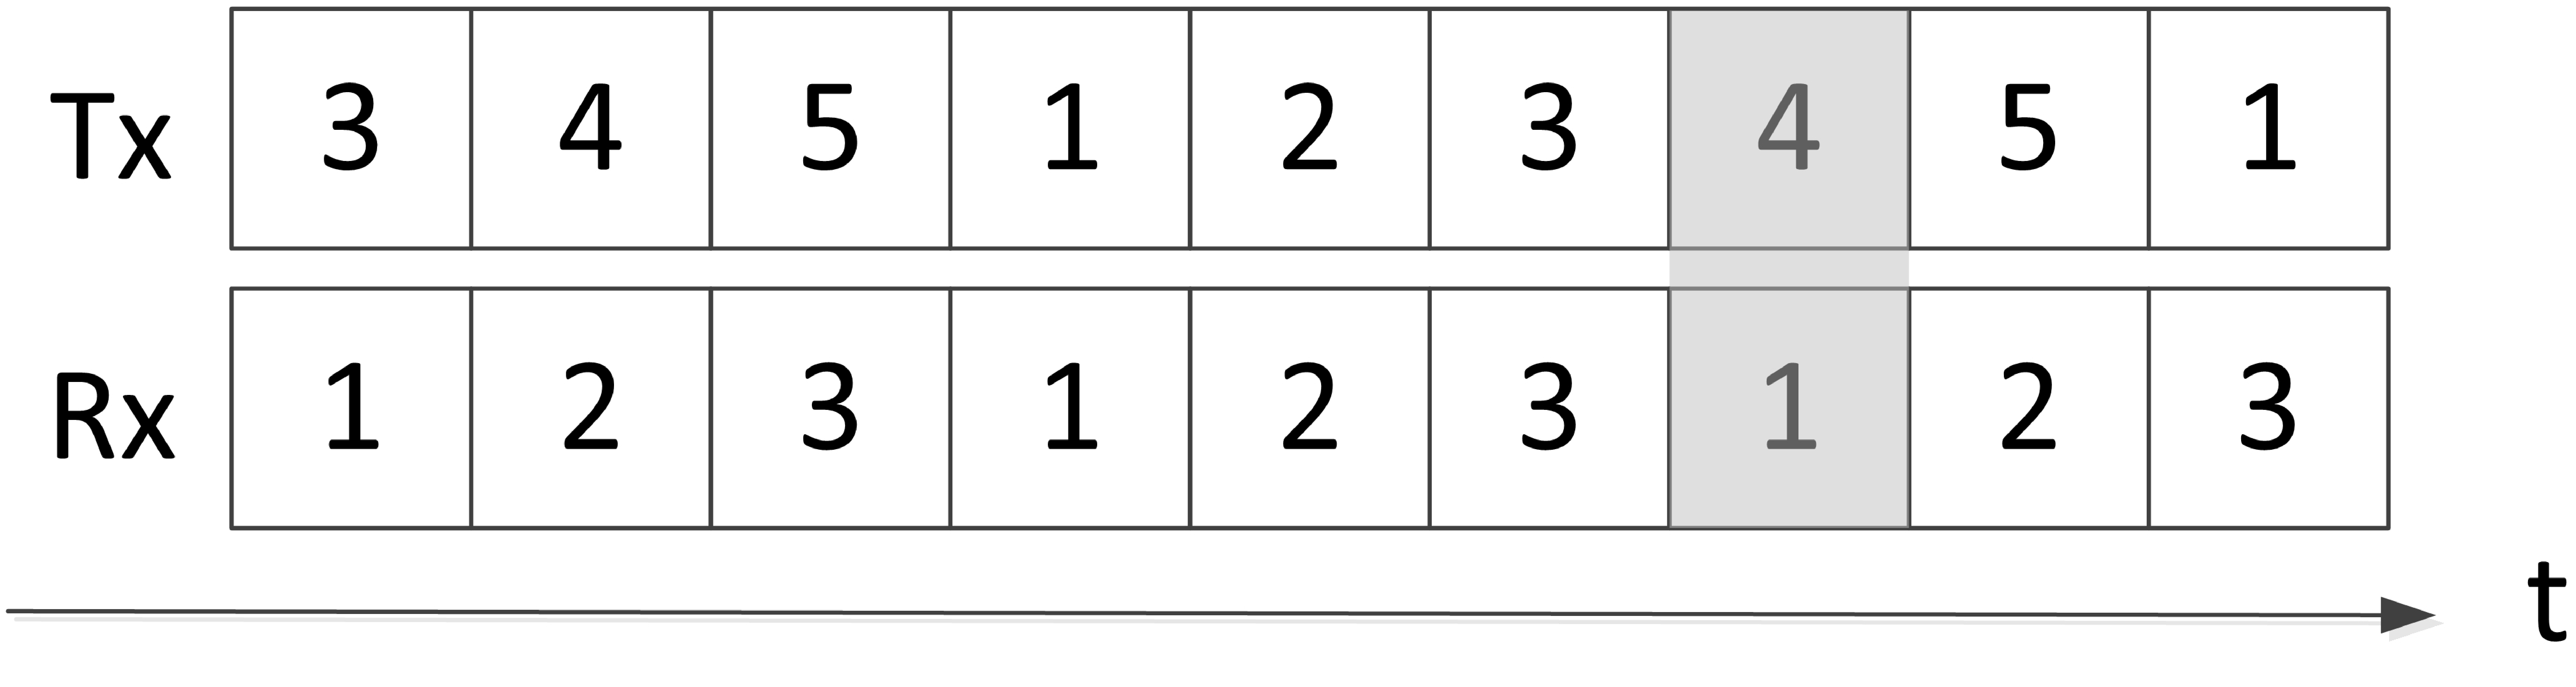
\includegraphics[width=8cm,height=2cm]{seq2.eps}
         \vspace{-0.2cm}
        \caption{An example of a rendezvous process under different sector numbers.} 
        \label{fig:example2}
    \end{center} 
\end{figure}

\addtocounter{theorem}{-2}
\begin{lemma}
\label{le:guarantee2}
If $P_{1} > P_{2}$ are two different prime numbers,  $x$ is a random number from $[0, P_{1}-1]$, the following $P_{1}$ numbers $x\%P_{1}+1$, $(x+P_{2})\%P_{1}+1$, $\dots$, $(x+(P_{1}-1)P_{2})\%P_{1}+1$ are all different.
\vspace{-0.2cm}
\end{lemma}
\begin{proof}
If there exist two different numbers $k_{1}\in [0, P_{1}-1], k_{2}\in [0, P_{1}-1]$ that $(x+k_{1}P_{2})\%P_{1}+1= (x+k_{2}P_{2})\%P_{1}+1$. Then, $[(k1-k2)P_{2}]\%P_{1} = 0$. As $P_{2}$ is a prime number, $P_{2}$ and $P_{1}$ are relatively prime. Therefore, $(k1-k2)\%P_{1} = 0$. Since $0\leq k_{1}< P_{1}, 0\leq k_{2}< P_{1}$, only when $k1 = k2$, $(k1-k2)\%P_{1} = 0$, which contradicts the assumption that $k_{1}\neq k_{2}$.
\end{proof}

\addtocounter{theorem}{1}
\begin{theorem}
\label{th:guarantee2}
If $N_{s}, N_{r}$ are different prime numbers and both SUs follow the sector hopping sequence generated from \textbf{Algorithm \ref{al:seq_rev}}, they can achieve a successful sector rendezvous within $N_{s}N_{r}$ sector hops.
\vspace{-0.2cm}
\end{theorem}
\begin{proof}
Without loss of generality, we assume that $N_{s} < N_{r}$, the sector rendezvous pair is $(p, q)$, and during the first round, when the SU sender is on the $p$th sector, the SU receiver is on the $\beta_{1} = \beta_{0}\%N_{r}+1$ sector, where $1\leq \beta_{0}\leq N_{r}$. According to \textbf{Algorithm \ref{al:seq_rev}}, during the next $N_{r}-1$ rounds, when the SU sender is on its $p$th sector, the SU receiver should be sequentially on $\beta_{2}=(\beta_{0}+N_{s})\%N_{r}+1, \beta_{3}=(\beta_{0}+2N_{s})\%N_{r}+1,\dots, \beta_{N_{r}}=[\beta_{0}+(N_{r}-1)N_{s}]\%N_{r}+1$. According to \textbf{Lemma \ref{le:guarantee2}}, the $N_{r}$ numbers $\beta_{1}, \beta_{2},\dots, \beta_{N_{r}}$ are all different. Therefore, there always exists a number $\beta_{t} = q$, where $1\leq t \leq N_{r}$. Since each sector hopping round contains $N_{s}$ sector hops, the maximum number of hops to guarantee a sector rendezvous is $N_{s}N_{r}$.
\end{proof}
\vspace{-0.2cm}
However, if the numbers of sectors of two SUs accidentally are the same prime number that $N_{s}=N_{r}$, the scheme we just proposed cannot work based on \textbf{Lemma \ref{le:guarantee2}}, while the scheme proposed in Section \ref{sec:equal} can work. In practice, the two SUs do not know each other's sector number before a successful sector rendezvous. How can they choose the scheme they should execute individually to guarantee a successful sector rendezvous? The solution is to combine the idea in this section and the one in Section \ref{sec:equal} together. For the SU receiver, it first adjusts the number of sectors $N_{r}$ to be the smallest prime number larger than the current one. Then, it generates a sector hopping sequence based on \textbf{Algorithm \ref{al:seq_rev}}. For the SU sender, it adjusts the number of sectors $N_{s}$ to be the smallest prime number larger than the current one. Next, it first generates a sector hopping sequence according to \textbf{Algorithm \ref{al:seq_send}}. After $N_{s}^{2}$ sector hops, if there is not a successful sector rendezvous, it generates the sector hopping sequence based on \textbf{Algorithm \ref{al:seq_rev}}. Based on this idea, we propose two distributed algorithms \textbf{Algorithm \ref{al:rend_rev}} and \textbf{Algorithm \ref{al:rend_send}} for the SU receiver and SU sender, respectively, considering both the indexing problem and the different sector number problem.
\begin{algorithm} 
  \caption{Sector rendezvous scheme for a SU receiver}
  \begin{algorithmic}[1] 
  \label{al:rend_rev}
    \REQUIRE ~~\\
    The number of sectors: $N_{r}$\\
    \IF{$N_{r}$ is not a prime number}
        \STATE Adjust $N_{r}$ to be the smallest prime number larger than it;
    \ENDIF
    \STATE Generate a sector hopping sequence based on \textbf{Algorithm \ref{al:seq_rev}} to perform the sector hopping process;
  \end{algorithmic} 
\end{algorithm}

\begin{algorithm} 
  \caption{Sector rendezvous scheme for a SU sender}
  \begin{algorithmic}[1] 
  \label{al:rend_send}
    \REQUIRE ~~\\
    The number of sectors: $N_{s}$\\
    \IF{$N_{s}$ is not a prime number}
        \STATE Adjust $N_{s}$ to be the smallest prime number larger than it;
    \ENDIF
    \STATE Generate a sector hopping sequence based on \textbf{Algorithm \ref{al:seq_send}} to perform the sector hopping process;
    \IF{No successful channel rendezvous after $N_{s}^{2}$ sector hops}
        \STATE Generate a sector hopping sequence based on \textbf{Algorithm \ref{al:seq_rev}} to perform the sector hopping process;
    \ENDIF
  \end{algorithmic} 
\end{algorithm}

Based on \textbf{Algorithm \ref{al:rend_rev}} and \textbf{Algorithm \ref{al:rend_send}}, we can get \textbf{Theorem \ref{th:guarantee3}}.
%\addtocounter{theorem}{1}
\begin{theorem}
\label{th:guarantee3}
Our proposed distributed schemes in \textbf{Algorithm \ref{al:rend_rev}} and \textbf{Algorithm \ref{al:rend_send}} can guarantee a successful sector rendezvous  within at most $N_{s}^{2}+N_{s}N_{r}$ sector hops, considering both the indexing problem and different sector number problem.
\vspace{-0.2cm}
\end{theorem}
\begin{proof}
After adjustments, $N_{s}$ and $N_{r}$ should be prime numbers. If $N_{s} = N_{r}$ after the adjustments, the two SUs can achieve a successful sector rendezvous within $N_{s}^{2}$ sector hops according to \textbf{Theorem \ref{th:guarantee1}}. If $N_{s} \neq N_{r}$ after the adjustments, the two SUs may not achieve a successful sector rendezvous within $N_{s}^{2}$ sector hops. Therefore, after $N_{s}^{2}$ sector hops, the SU sender can realize that $N_{s} \neq N_{r}$ and then generates a sector hopping sequence based on \textbf{Algorithm \ref{al:seq_rev}}. According to \textbf{Theorem \ref{th:guarantee2}}, during the next $N_{s}N_{r}$ sector hops, two SUs can achieve a successful sector rendezvous. Therefore, two SUs can achieve a successful sector rendezvous within at most $N_{s}^{2}+N_{s}N_{r}$ sector hops, considering all scenarios.
\end{proof}

\section{Power Control Protocol to Maximize The Number of Common Available Channels}
\subsection{Problem Description} 
\label{sec:des} 
\vspace{-0.1cm} Consider two SUs in a CRAHN: one is the sender and the other is the receiver during  
a transmission. For the SU sender, its transmission on a channel may generate direct  
interference to the PUs who are using the same channel. Thus, the sensing threshold  
of a SU sender should be set to guarantee the interference generated from it is low  
enough to the PUs outside the sensing range. However, for the SU receiver, it does  
not generate direct interference to any PU, but its reception may be interfered by a  
PU's transmission on the same channel. The SU receiver's sensing threshold should  
guarantee its received signal not be interfered seriously by PUs' transmission on the  
same channel. Therefore, the sensing threshold of the SU sender and receiver could  
be different because of their different roles in the communication. Now, the problem  
is: how to determine the optimal sensing threshold for both the SU sender and receiver?   
To solve this problem, we first show the relationship between the sensing threshold,  
sensing range, and transmission power for the SU sender and SU receiver in the following. 
\subsection{Analysis of the Sensing Range of a SU Sender} 
\vspace{-0.2cm} The requirement that a SU sender can sense whether there is an interfering transmission  
power on channel $i$ is that the sensed power from channel $i$ should be larger than a  
threshold $P_{th\_su\_s}$ \cite{fDigham03OTEDO}. %cite energy sensing papers% 
The relationship between the sensing threshold and $P_{th\_su\_s}$ can be formulated by 
using the widely used transmission model \cite{aGoldsmith05WC,yHou08SSFMN} that
\begin{equation} 
  P_{th\_su\_s} =  \DF{P_{pu}\kappa_{1}}{r_{su\_s}^{\alpha}}, \label{1} 
\end{equation} 
where $P_{pu}$ is the transmission power of a PU, $\kappa_{1}$ is an antenna  
related constant, $\alpha$ is the path-loss factor, and $r_{su\_s}$ is the sensing  
range of the SU sender. Equation (1) shows that the sensing range is determined  
by the sensing threshold. 

\vspace{-0.2cm} Moreover, for the SU sender, it cannot use channel $i$  
when its transmission power on channel $i$ produces an unacceptable interference  
to a PU receiver. According to the definition of the sensing range, we can get 
\begin{equation} 
  \DF{P_{su}\kappa_{2}}{r_{su\_s}^{\alpha}} \leq P_{pu\_min}, \label{2} 
\end{equation} 
where $P_{su}$ is the transmission power of the SU sender and $P_{pu\_min}$ is the  
highest acceptable interference power on channel $i$ for a PU receiver which can be  
obtained by the PU's minimum required decoding power and signal-to-interference  
ratio (SIR). From \eqref{2}, we can get the minimum sensing range of a SU sender 
\begin{equation} 
  r_{su\_s\_min} = \left(\DF{P_{su}\kappa_{2}}{P_{pu\_min}}\right)^{\frac{1}{\alpha}}.\label{3} 
\end{equation} 

\vspace{-0.2cm} For a SU, a larger sensing range means more unavailable channels and less available  
channels. Thus, we can use the minimum sensing range in \eqref{3} to set the threshold  
in \eqref{1} for the sensing process of a SU sender which can also guarantee an acceptable  
interference to PU receivers. 
\subsection{Analysis of the Sensing Range of a SU Receiver} 
For a SU receiver, its sensing range also has a similar relationship as in \eqref{1} with  
its detection threshold  
\begin{equation} 
  P_{th\_su\_r} =  \DF{P_{pu}\kappa_{3}}{r_{su\_r}^{\alpha}}, \label{4} 
\end{equation} 
where $P_{th\_su\_r}$ is the sensing detection threshold of the SU receiver, $P_{pu}$ is  
the transmission power of a PU, and $r_{su\_r}$ is the sensing range of the SU receiver.  
However, a SU receiver cannot judge whether it can use channel $i$ simply based on  
whether the sensed power on channel $i$ is higher than 
$P_{th\_su\_r}$, because the received signal power from the SU sender may be  
much higher than the interference power. Accordingly, the SU receiver should  
additionally check if the received signal from the SU sender can meet the minimum  
required SIR that 
\begin{equation} 
  \DF{P_{su\_rev}}{P_{th\_su\_r}} \geq SIR_{su\_min},\label{5} 
\end{equation} 
where $P_{su\_rev}$ is the received SU power from channel $i$, $P_{th\_su\_r}$ is the  
sensing detection threshold for the SU receiver, and $SIR_{su\_min}$ is the minimum  
required SIR for correctly decoding. We ignore the environment noise here. 
 $P_{su\_rev}$ can be obtained by 
\begin{equation} 
  P_{su\_rev} = \DF{P_{su}\kappa_{4}}{d_{su}^{\alpha}},\label{6} 
\end{equation} 
where $d_{su}$ is the distance between the SU sender and SU receiver.  
From \eqref{4}\eqref{5}\eqref{6}, we can get the minimum sensing range of the SU receiver 
\begin{equation} 
  r_{su\_r\_min} = \left(\DF{P_{pu}\kappa_{3} 
  SIR_{su\_min}d_{su}^{\alpha}}{P_{su}\kappa_{4}}\right)^{\frac{1}{\alpha}}. \label{7} 
\end{equation} 
From a SU receiver's angle, in order to get more available channels, we can  
use the minimum sensing range in \eqref{7} as the SU receiver's sensing range  
to determine its sensing threshold by using \eqref{4}. 

\vspace{-0.2cm} The sensing range of a SU will directly affect the number of its individual available channels.  
 Equation \eqref{3}  and \eqref{7} indicate  
that when the transmission power of the SU sender $P_{su}$ decreases, the sensing  
range of the SU sender will decrease but the sensing range of the SU receiver will  
increase, and vice versa. Thus, there is a trade-off between the SU transmission power  
and the sensing range of the SU pair which is also related to their individual available  
channels. How to determine the optimal SU transmission power which can result in the  
maximum number of common available channels for a SU pair in CRAHNs is an important  
issue that may affect the performance of SU transmissions.  
In the next section, we use the SU sensing ranges to estimate the expectation of the  
number of common available channels between two SUs and then determine the  
optimal SU transmission power to maximize the number of common available channels. 
\subsection{System Model} 
\label{sec:sys} 
\vspace{-0.2cm} We consider two SUs in an area whose size is $S = L \times L$. One SU is the SU  
sender $SU_{1}$, while the other SU is the SU receiver $SU_{2}$. The set of all  
channels is $\mathcal{\mathcal{M}}=\{1,2,\dots ,M\}$ which has $M$ channels. 
We assume that all the $N$ PUs are evenly distributed in the whole area. Their  
active probability is $\beta$.  Each PU randomly chooses a channel to transmit,  
and its traffic follows the exponential distribution. 

\subsection{The Expectation of the Number of Common Available Channels} 
\vspace{-0.2cm} In Fig. 1, the two circles represent the sensing range of $SU_{1}$ or $SU_{2}$.  
The combined area of their sensing ranges $A_{0}$ has three parts: $A_{1}$, $A_{2}$,  
and $A_{3}$, and their sizes are $S_{0}$, $S_{1}$, $S_{2}$, and $S_{3}$, respectively. 
\begin{figure}[hbtp] 
\vspace{-1em}
\setlength{\abovecaptionskip}{-0.1cm}
    \begin{center} 
        \includegraphics[width=6cm,height=4cm]{sen_range.jpg} 
        \caption{The sensing range of the SU sender and receiver.} 
        \label{fig:sen_ranges} 
    \end{center}  
    \vspace{-1.5em}
\end{figure}

\vspace{-0.2cm} Let $\mathcal{M}_{u\_s}$ be the set of the channels which cannot be used  
by the SU sender, $\mathcal{M}_{u\_r}$ be the set of channels which cannot  
be used by the SU receiver, and $\mathcal{M}_{c}$ be the set of common  
available channels of the SU pair. Thus, we have 
\begin{equation} 
\mathcal{M}_{c} = \mathcal{M} - ( \mathcal{M}_{u\_s} \bigcup \mathcal{M}_{u\_r} ).\label{8} 
\end{equation} 
Let $\mathcal{M}_{used} = \mathcal{M}_{u\_s} \bigcup \mathcal{M}_{u\_r}$ be the set  
of channels which has been used by the PUs within the sensing range of $SU_{1}$  
and $SU_{2}$. Accordingly, the expectation of the number of common available  
channels of $SU_{1}$ and $SU_{2}$ is 
\begin{equation} 
    E[|\mathcal{M}_{c}|] = |\mathcal{M}| - E[|\mathcal{M}_{used}|], \label{9} 
\end{equation} 
where $|\bullet|$ means the size of a set. 

\vspace{-0.2cm} We use a similar method as shown in \cite{ySong11AQBPF} 
to calculate $E[|\mathcal{M}_{used}|]$. Since PUs are evenly distributed in the  
whole area, the probability that there are $k$ PUs in $A_{0}$ is: 
\begin{equation} 
P(n=k) = \binom{N}{k}\left( \DF{S_{0}}{S}\right) ^{k}\left(1-\DF{S_{0}}{S}\right)^{N-k}.\label{10} 
\end{equation} 
When the active probability of PUs is $\beta$, the probability that there are $i$ concurrent  
active PUs among all the $k$ PUs in $A_{0}$ is: 
\begin{equation} 
P(v=i|n=k) = \binom{k}{i}\beta^i\left(1-\beta\right)^{(k-i)}.\label{11} 
\end{equation} 
 Next, we calculate the probability that there are $j$ used channels while
  $i$ active PUs in $A_{0}$. Since each PU randomly chooses a channel  
 among all $M$ channels with the same probability, this problem is equivalent  
 to randomly putting $i$ different balls into $M$ different boxes and finding  
 the probability of $j$ non-empty boxes. The answer to this problem is: 
\begin{equation} 
P(u=j|v=i)=\DF{\binom{M}{j}S(i,j)j!}{M^{i}}, \label{12} 
\end{equation} 
where $S(i,j)$ is the Stirling number which represents the number of different  
ways to split $i$ different elements into $j$ different non-empty sets.  
From \eqref{10}, \eqref{11}, and \eqref{12}, we can get the average number  
of the used channels  as shown in \eqref{13} in the next page.  Therefore, according to \eqref{9}, in order to maximize the  expectation of the number of common available channels, we should find the optimal $P_{su}$ that  
minimizes $E[|\mathcal{M}_{used}|]$. 
\newcounter{mytempeqncnt} 
\begin{figure*}[!t] 
% ensure that we have normalsize text 
\normalsize 
% Store the current equation number. 
%\setcounter{mytempeqncnt}{\value{equation}} 
% Set the equation number to one less than the one 
% desired for the first equation here. 
% The value here will have to changed if equations 
% are added or removed prior to the place these 
% equations are referenced in the main text. 
%\setcounter{equation}{12} 
\begin{equation} 
\label{13} 
E[|\mathcal{M}_{used}|]=\sum_{k=0}^{N}\sum_{i=0}^{k}\sum_{j=0}^{i}j\ 
\binom{N}{k}\left( \DF{S_{0}}{S}\right) ^{k}\left(1-\DF{S_{0}}{S}\right)^{N-k}\ 
\binom{k}{i}\beta^i\left(1-\beta\right)^{k-i}\ 
\DF{\binom{M}{j}S(i,j)j!}{M^{i}} 
\end{equation} 
% Restore the current equation number. 
%\setcounter{equation}{\value{mytempeqncnt}} 
% IEEE uses as a separator 
\hrulefill 
% The spacer can be tweaked to stop underfull vboxes. 
\vspace*{4pt} 
\end{figure*} 
\subsection{The Optimization Solution} 
\vspace{-0.2cm} From the above derivations, it is very challenging to get an explicit expression  
for the optimal $P_{su}$. We propose an approximation solution for the optimization  
problem. This solution is easy to implement in designing a practical power control  
protocol and can produce an improvement in the throughput according to the  
simulation results shown in Section \ref{sec:simu}. 

\vspace{-0.2cm} Let $E[|\mathcal{M}_{used}|]$ be a function of $\frac{S_{0}}{S}$, named $f(x)$. 
\begin{lemma} 
$f(x_{1}) \geq f(x_{2})$  when $x_{1} \geq x_{2}$ and $N > 1$.\label{lemma1} 
\end{lemma} 
\begin{proof} 
We can rewrite $f(x)$ as: 
\begin{align*} 
f(x) &=\sum_{k=0}^{N}\binom{N}{k}x^{k}(1-x)^{N-k}g(k),\\ 
g(k) &= \sum_{i=0}^{k}\binom{k}{i}\beta^{i}\left(1-\beta\right)^{k-i}q(i),\\ 
q(i) &= \sum_{j=0}^{i}jp(j),\\ 
p(j) &=\DF{\binom{M}{j}S(i,j)j!}{M^{i}}. 
\end{align*} 
According to the definition of $p(j)$, we can get $\sum_{j=0}^{i}p(j)=1$. Thus, we  
can induce that when $i > 1, q(i) = \sum_{j=0}^{i}jp(j) > \sum_{j=0}^{i}p(j) = 1$.  
Let $g(k) = \sum_{i=0}^{k}\binom{k}{i}\beta^{i}\left(1-\beta\right)^{k-i}t$,  
where $t$ is a constant. If $t \leq 1$ then $\sum_{i=0}^{k}\binom{k}{i}\beta^i\left(1-\beta\right)^{k-i}t <  
\sum_{i=0}^{k}\binom{k}{i}\beta^{i}\left(1-\beta\right)^{k-i}q(i)$,  
because $q(i) > 1$ when $i > 1$. This is a paradox. Therefore, $t > 1$  
when $k > 1$. Then, we can rewrite  
 $g(k) = \sum_{i=0}^{k}\binom{k}{i}(t^{\frac{1}{i}}\beta)^{i}\left(1-\beta\right)^{k-i} 
 = ( t^{\frac{1}{i}}\beta + 1 - \beta)^{k}$. According to the definition,  
 $0<\beta <1$, then we can get $g(k) > 1$ when $k > 1$. Repeat the same steps,  
 we can also rewrite $f(x)$ as  
 $f(x) =\sum_{k=0}^{N}\binom{N}{k}x^{k}(1-x)^{N-k}l$, where $l > 1$  
 when $N > 1$. 
 Last, we can get the final expression of $f(x)$ as  
 $f(x) = \sum_{k=0}^{N}\binom{N}{k}(l^{\frac{1}{k}}x)^{k}(1-x)^{N-k} =  
 (l^{\frac{1}{k}}x + 1 - x)^{N}$. Since $l > 1$ when $N > 1$, we can finally  
 conclude that $f(x)$ increases if $x$ increases. 
\end{proof} 
From Lemma 1, we can know that in order to minimize  
$E[|\mathcal{M}_{used}|]$, we should minimize the area size $S_{0}$.  
Now consider the following problem: there are two circles $C_{0}$ and $C_{1}$  
whose radii are $r_{0}$ and $r_{1}$.  
Their distance is larger than zero and does not change. Their radii only change simultaneously  
with a constant rate $c$ and $-c$. Let \textit{s} be the size of their combination  
area, then we can get the following lemma: 
\begin{lemma} 
When $r_{0} = r_{1}$, $s$ will be minimum.\label{lemma2} 
\end{lemma} 
\vspace{-0.1in} 
\begin{proof} 
Assume $r_{1}$ increases from $0$ to the maximum value $r_{max}$.  
As the radius changes with a constant but opposite rate, $r_{0}$ decreases 
from $r_{max}$ to $0$. Let $s=G(r_{0})$. We can get that $G(x)$ is symmetric 
according to the axis $x=\frac{1}{2}r_{max}$, since 
$r_{0}$ and $r_{1}$ change simultaneously with a constant but opposite rate. 
When $r_{0}$ decreases from $r_{max}$ to $\frac{1}{2}r_{max}$, $G(x)$  
also decreases. Because when $r_{0} > r_{1}$ and they change simultaneously  
with a constant but opposite rate, the size that $C_{0}$ decreases is larger than  
the size that $C_{1}$ increases. Furthermore, according to the symmetry  
of $G(x)$, when $r_{0}$ decreases from 
$\frac{1}{2}r_{max}$ to $0$, $G(x)$ increases. Thus, when $r_{0}=\frac{1}{2}r_{max}$  
and $r_{1}$ is also $\frac{1}{2}r_{max}$,  $G(x)$ will reach its minimum value.  
\end{proof} 
According to Equation \eqref{3} and \eqref{7}, when $P_{su}$ increases, $r_{su\_s\_min}$  
will increase and $r_{su\_r\_min}$ will decrease, and vice versa. Using Lemma  
\ref{lemma1} and Lemma \ref{lemma2}, we can get an approximate optimal  
$P_{su}$ by assuming $r_{su\_s\_min}$ and $r_{su\_r\_min}$ change with a  
constant but opposite rate. Therefore, letting Equation \eqref{3} equal \eqref{7},  
the final expression of the approximately optimal SU transmission power is 
\begin{equation} 
P_{su\_opt} = \sqrt{\DF{P_{pu\_min}P_{pu}SIR_{su\_min}d_{su}^{\alpha}\kappa_{3}} 
{\kappa_{2}\kappa_{4}}}. \label{eq:su_t_opt} 
\end{equation} 

\vspace{-0.2cm} Fig. \ref{fig:opt_val} shows the minimum values of $E[|\mathcal{M}_{used}|]$ when the real 
optimal $P_{su}$ is used (which is obtained by the numerical method)  
and the results using our approximate optimal $P_{su}$ solution, when the distance between two SUs 
changes from $5m$ to $15m$. We can see that  the two results coincide very well, 
which means that our approximate optimal solution is valid and applicable. 
\begin{figure}[hbtp] 
\vspace{-0.4cm}
\setlength{\abovecaptionskip}{-0.1cm}
    \begin{center} 
        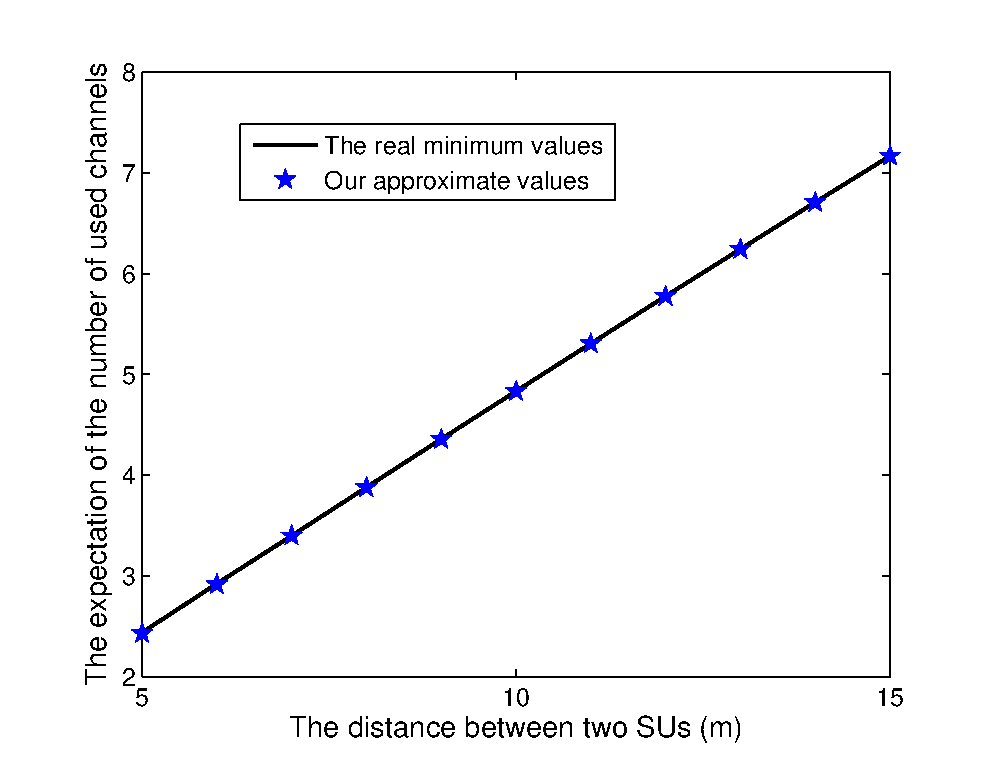
\includegraphics[width=6cm,height=5cm]{opt_val.eps} 
        \caption{The real minimum values and our approximate values.} 
        \label{fig:opt_val} 
    \end{center} 
    \vspace{-1.5em} 
\end{figure} 

\subsection{The Proposed Power Control Protocol} 
\label{sec:pro} 
\vspace{-0.2cm} In order to implement the optimization solution, we make the following assumptions.  
We assume that each SU is equipped with a GPS to get its own coordinates.  
Moreover, according to our proposed algorithms, the SU pair should know some  
parameters of each other. How to get these parameters without a common control  
channel in CRAHNs is a challenge. In wireless ad-hoc networks, a sender and the  
receiver use the Request-to-Send (RTS) and Clear-to-Send (CTS) packets to inform  
each other before transmitting data packets. Thus, we can insert the needed information  
into the RTS and CTS packets.   
We assume that the SUs use the common hopping method in \cite{ySong12APSHF} to achieve successful  
rendezvous and the RTS and CTS packets exchange.  
Under this method, two SUs follow the same hopping sequence to perform  
channel hopping in each time slot. When one  
SU wants to send packets to the other, it sends the RTS packet on the currently  
staying channel. After receiving the CTS packet from the other SU in the later  
time slot, it sends data packets to the SU receiver. 


\vspace{-0.2cm} In order to implement our  
proposed power control protocol, we design the algorithms for the SU sender  
and SU receiver. When the SU sender wants to send packets to the SU receiver,  
it will execute Algorithm 1. After receiving the RTS packet, the SU receiver will  
execute Algorithm 2. During the execution of the algorithms, they use the  
calculated optimal transmission power to get the corresponding sensing range  
and sensing threshold. From the pseudo code of 
Algorithm 1 and Algorithm 2, we can see that the complexity is $O(1)$. Thus, our  
algorithm has a low time cost and is easy to implement. 
\vspace{-0.2cm} 
\begin{algorithm} 
  \caption{The algorithm for the SU sender} 
  \begin{algorithmic}[1] 
    \REQUIRE ~~\\ 
      Its coordinates $(X_{su\_s},Y_{su\_s})$;\\ 
      $\kappa_{1}$, $\kappa_{2}$, $\alpha$, $P_{pu}$, and $P_{pu\_min}$; 
    \ENSURE ~~\\ 
      Its optimal sensing threshold $P_{th\_su\_s\_opt}$;\\ 
      Its optimal transmission power $P_{su\_opt}$;\\ 
    \STATE Add $X_{su\_s}$ and $Y_{su\_s}$ into the RTS packet; 
    \STATE Send the RTS packet; 
    \STATE After receiving the returned CTS packet, get the optimal transmission\ 
           power $P_{su\_opt}$ from the CTS packet; 
    \STATE Use $P_{su\_opt}$ and Equation \eqref{3} to determine its optimal\ 
           sensing range $r_{su\_s\_opt}$; 
    \STATE Use $r_{su\_s\_opt}$ and Equation \eqref{1} to determine its \ 
           optimal sensing threshold $P_{th\_su\_s\_opt}$; 
    \STATE Reset its sensing threshold as $P_{th\_su\_s\_opt}$ and transmission  
    power as $P_{su\_opt}$; 
  \end{algorithmic} 
\end{algorithm} 
\begin{algorithm}[htb] 
  \caption{The algorithm for the SU receiver} 
  \begin{algorithmic}[1] 
    \REQUIRE ~~\\ 
    $\kappa_{2}$, $\kappa_{3}$, $\kappa_{4}$, $\alpha$, and $P_{pu}$;\\ 
    Its minimum required SIR: $SIR_{min}$;\\ 
    The RTS packet from the SU sender; 
    \ENSURE ~~\\ 
    The SU sender's optimal transmission power $P_{su\_opt}$;\\ 
    Its optimal sensing threshold $P_{th\_su\_r\_opt}$;\\ 
    \STATE Get $X_{su\_s}$ and $Y_{su\_s}$ from the RTS packet, and its own coordinates  
           $X_{su\_r}$ and $Y_{su\_r}$from its GPS; 
    \STATE  Use $d_{su}=\sqrt{(X_{su\_s} - X_{su\_r})^2 + (Y_{su\_s} - Y_{su\_r})^2}$  
    to calculate the distance to the SU sender; 
    \STATE Use \eqref{eq:su_t_opt} to get 
           the optimal transmission power $P_{su\_opt}$; 
    \STATE Use $P_{su\_opt}$ and Equation \eqref{7}  to determine\ 
           its optimal sensing range $r_{su\_r\_opt}$; 
     \STATE Use $r_{su\_r\_opt}$ and Equation \eqref{4}  to determine\ 
           its optimal sensing threshold $P_{th\_su\_r\_opt}$; 
     \STATE Reset its sensing threshold as $P_{th\_su\_r\_opt}$; 
     \STATE Insert $P_{su\_opt}$ to the CTS packet and send it; 
  \end{algorithmic} 
\end{algorithm} 
\chapter{Conclusion and Future Work}
\section{Conclusion of Completed Work}
\section{Future Work}
\section{Publications}


\fbmatterchapterformat

\bibliographystyle{ieeetr}
\bibliography{ji-li-all-references}


\end{document}
